%%%%%%%%%%%%%%%%%%%%%%%%%%%%%%%%%%%%%%%%%%%%%%%%%%%%%%%%
%%%%%%%%%%%%%%%%%%%%%%%%%%%%%%%%%%%%%%%%%%%%%%%%%%%%%%%%
%%%%%%%%%%%%%%%%%%%%%%%%%%%%%%%%%%%%%%%%%%%%%%%%%%%%%%%%
\chapter{General Machine Learning (ML) Concepts}
\label{chap:ml_general}

%%%%%%%%%%%%%%%%%%%%%%%%%%%%%%%%%%%%%%%%%%%%%%%%%%%%%%%%
%%%%%%%%%%%%%%%%%%%%%%%%%%%%%%%%%%%%%%%%%%%%%%%%%%%%%%%%
\section{Supervised Learning}
\label{ml_general:supervised}

In supervised learning a model is trained over many known examples
to use input features $\mb{X}$ to make a prediction \yhat about the true value $y$.
During the training process parameters $\beta$ of
the model are adjusted to minimize a two-part objective function,
$S\left(\beta\right) = L\left(\beta\right) + \Omega\left(\beta\right)$.
The training loss $L\left(\beta\right)$ measures the model's predictive performance
while $\Omega\left(\beta\right)$ is a regularization term to penalize model complexity.
Note that $L$ is a measure of the model's bias,
while $\Omega$ is --- somewhat --- a measure of its variance,
so $S\left(\beta\right)$ captures both parts of the bias-variance tradeoff \cite{HastieTF09}.

%%%%%%%%%%%%%%%%%%%%%%%%%%%%%%%%%%%%%%%%%%%%%%%%%%%%%%%%
%%%%%%%%%%%%%%%%%%%%%%%%%%%%%%%%%%%%%%%%%%%%%%%%%%%%%%%%
\section{Unsupervised Learning}
\label{ml_general:unsupervised}
% TODO

%%%%%%%%%%%%%%%%%%%%%%%%%%%%%%%%%%%%%%%%%%%%%%%%%%%%%%%%
%%%%%%%%%%%%%%%%%%%%%%%%%%%%%%%%%%%%%%%%%%%%%%%%%%%%%%%%
\section{Evaluating Performance}
\label{ml_general:eval}
% TODO

%%%%%%%%%%%%%%%%%%%%%%%%%%%%%%%%%%%%%%%%%%%%%%%%%%%%%%%%
\subsection{Cross-Validation}
\label{ml_general:eval:cv}
% TODO

%%%%%%%%%%%%%%%%%%%%%%%%%%%%%%%%%%%%%%%%%%%%%%%%%%%%%%%%
\subsection{Confusion Matrix}
\label{ml_general:eval:cm}

The confusion matrix is a simple table of the number of actual, or truth, class instances
versus the number of a model's predicted class instances.
A two class example is provided in \cref{table:CM}.
Multi-class confusion matrices are straight forward extensions,
with correctly classified instances appearing along the diagonal.

\begin{table}[H]
  \centering
  \begin{tabular}{c | c | c | c |}
  \multicolumn{2}{c}{} & \multicolumn{2}{c}{\textbf{Actual}} \\ \cline{3-4}
  \multicolumn{1}{c}{} & & Positive & Negative \\ \cline{2-4}
  \multirow{4}{*}{\rotatebox{90}{\textbf{Predicted}}} & \multirow{2}{*}{Positive} & \multirow{2}{*}{TP} & FP \\[-8pt]
   & & & (Type I or $\alpha$) \\ \cline{2-4}
   & \multirow{2}{*}{Negative} & FN & \multirow{2}{*}{TN} \\[-8pt]
   & & (Type II or $\beta$) & \\ \cline{2-4}
  \end{tabular}
  \caption{Two class confusion matrix.}
  \label{table:CM}
\end{table}

%%%%%%%%%%%%%%%%%%%%%%%%%%%%%%%%%%%%%%%%%%%%%%%%%%%%%%%%
\subsection{TPR \& TNR -- Sensitivity \& Specificity}
\label{ml_general:eval:TPR_TNR}

The true positive rate (TPR) and true negative rate (TNR) are
relatively straight forward to compute and understand, along with their complements,
the false negative rate (FNR), \ie miss rate, and false positive rate (FPR), \ie fall-out.
Here the denominators are the number of true class members.

\begin{enumerate}[noitemsep]
  \item True positive rate (TPR), \ie sensitivity, recall, hit rate:
\begin{equation} \label{eq:TPR}
\text{TPR} = \frac{\text{TP}}{\text{P}} = \frac{\text{TP}}{\text{TP}+\text{FN}} = 1 - \text{FNR} = P\left(\hat{+} \mid + \right)
\end{equation}

  \item True negative rate (TNR), \ie specificity, selectivity:
\begin{equation} \label{eq:TNR}
\text{TNR} = \frac{\text{TN}}{\text{N}} = \frac{\text{TN}}{\text{TN}+\text{FP}} = 1 - \text{FPR} = P\left(\hat{-} \mid - \right)
\end{equation}
\end{enumerate}

%%%%%%%%%%%%%%%%%%%%%%%%%%%%%%%%%%%%%%%%%%%%%%%%%%%%%%%%
\subsection{PPV (Precision) \& NPV}
\label{ml_general:eval:PPV_NPV}

The positive predictive value (PPV), more commonly known as precision, and negative predictive value (NPV)
are related metrics, but with predicted class members in the denominators.
Their complements are the false discovery rate (FDR) and false omission rate (FOR).
It is helpful to look at these metrics graphically, as in \cref{fig:graphical_CM_quantities}.

\begin{enumerate}[noitemsep]
  \item Positive predictive value (PPV), \ie precision:
\begin{equation} \label{eq:PPV}
\text{PPV} = \frac{\text{TP}}{\hat{\text{P}}} = \frac{\text{TP}}{\text{TP}+\text{FP}} = 1 - \text{FDR} = P\left(+ \mid \hat{+} \right)
\end{equation}

  \item Negative predictive value (NPV):
\begin{equation} \label{eq:NPV}
\text{NPV} = \frac{\text{TN}}{\hat{\text{N}}} = \frac{\text{TN}}{\text{TN}+\text{FN}} = 1 - \text{FOR} = P\left(- \mid \hat{-} \right)
\end{equation}
\end{enumerate}

\begin{figure}[H]
\centering
  \begin{subfigure}[c]{0.48\textwidth}\centering
  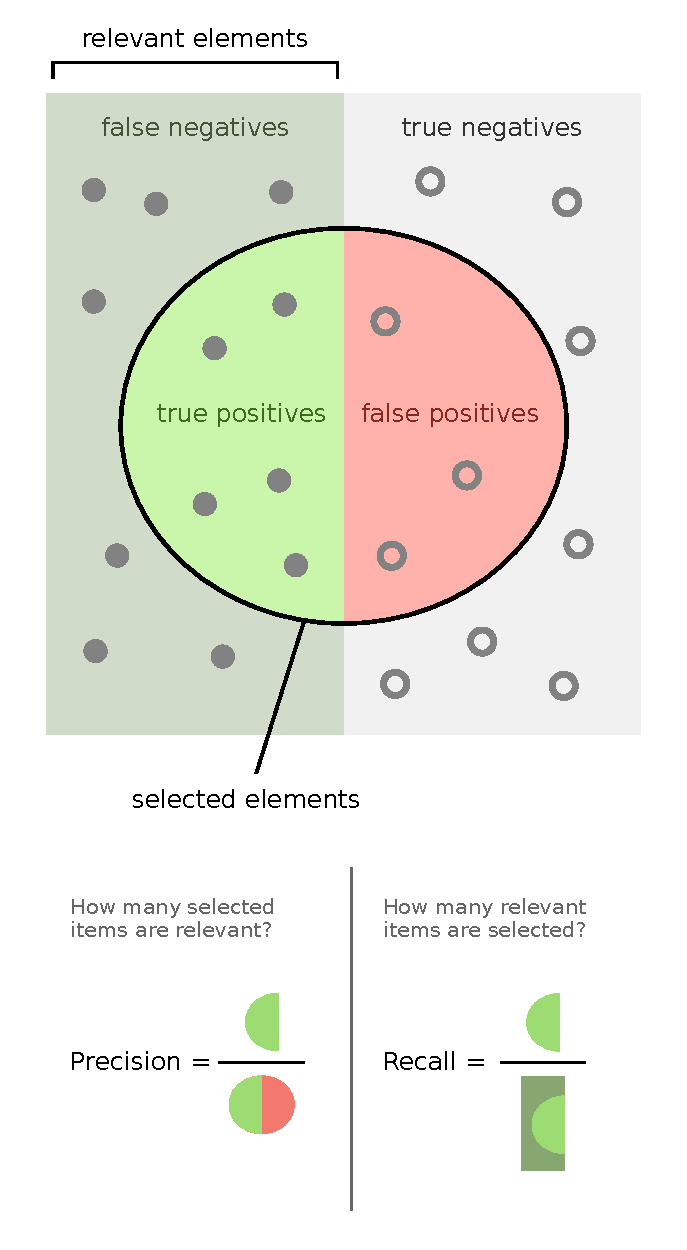
\includegraphics[width=\textwidth]{figures/ml/precision_recall}
  \caption{Precision \& Recall}
  \label{fig:graphical_CM_quantities:precision_recall}
  \end{subfigure}
  ~
  \begin{subfigure}[c]{0.48\textwidth}\centering
  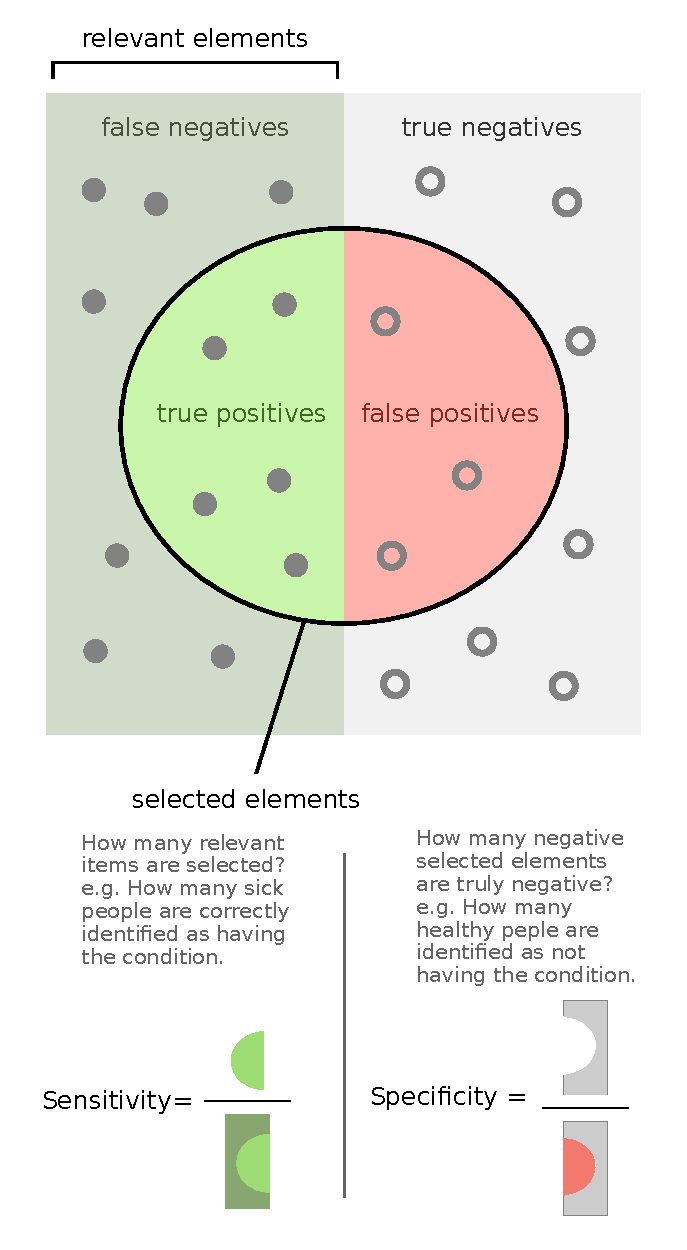
\includegraphics[width=\textwidth]{figures/ml/sensitivity_and_specificity}
  \caption{Sensitivity \& Specificity}
  \label{fig:graphical_CM_quantities:sensitivity_specificity}
  \end{subfigure}
\caption{
Graphical representation of
precision versus recall (sensitivity), by \href{https://commons.wikimedia.org/wiki/File:Precisionrecall.svg}{Walber},
and
sensitivity (recall) versus specificity, by \href{http://en.wikipedia.org/wiki/File:Sensitivity_and_specificity.svg}{FeanDoe}.
}
\label{fig:graphical_CM_quantities}
\end{figure}

%%%%%%%%%%%%%%%%%%%%%%%%%%%%%%%%%%%%%%%%%%%%%%%%%%%%%%%%
\subsection{Cohen's \texorpdfstring{$\kappa$}{Kappa}}
\label{ml_general:eval:cohens_kappa}
% TODO

\begin{subequations} \label{eq:cohens_kappa}
\begin{align}
\kappa &= \frac{p_{o} - p_{e}}{1-p_{e}} = 1 - \frac{1-p_{o}}{1-p_{e}} \label{eq:cohens_kappa:def} \\
&= 2\, \frac{\text{TP} \times \text{TN} - \text{FP} \times \text{FN} }{ \left(\text{TP} + \text{FP}\right) \times \left(\text{FP} + \text{TN}\right) \times \left(\text{TP} + \text{FN}\right) \times \left(\text{FN} + \text{TN}\right) } \label{eq:cohens_kappa:cm} \\
p_{e} &= \frac{1}{N^{2}} \sum_{k} n_{k1} n_{k2} \label{eq:cohens_kappa:pe}
\end{align}
\end{subequations}

%%%%%%%%%%%%%%%%%%%%%%%%%%%%%%%%%%%%%%%%%%%%%%%%%%%%%%%%
\subsection{Other Scores}
\label{ml_general:eval:other_scores}

The accuracy (ACC), the proportion of correct predictions, is a natural metric for measuring a classifiers performance.
Various $F$-scores, such as $F_{1}$ and $F_{\beta}$, combine precision and recall
into one metric\footnote{Note that $F_{\beta}$ does not depend on TN at all, a benefit with imbalanced classes.}.
$F_{1}$ balances precision and recall equally, and is their harmonic mean,
while $F_{\beta}$ uses $\beta$ to assign different weights to each\footnote{$F_{2}$ weights recall over precision, $F_{0.5}$ weights precision over recall.}.

\begin{enumerate}[noitemsep]
  \item Accuracy (ACC):
\begin{equation} \label{eq:ACC}
\text{ACC} = \frac{\text{TP}+\text{TN}}{\text{P}+\text{N}} = \frac{\text{TP}+\text{TN}}{\text{TP}+\text{TN}+\text{FP}+\text{FN}}
\end{equation}

  \item $F_{1}$ ($F_{1}=1$ is best, $F_{1}=0$ is worst):
\begin{equation} \label{eq:F1}
F_{1} = \left(\frac{\text{precision}^{-1}+\text{recall}^{-1}}{2}\right)^{-1} = 2\,\,\frac{\text{precision} \times \text{recall}}{\text{precision} + \text{recall}}
\end{equation}

  \item $F_{\beta}$ (Larger $\beta$ weights recall over precision):
\begin{equation} \label{eq:Fbeta}
F_{\beta} = \left(1+\beta^{2}\right) \frac{\text{precision} \times \text{recall}}{\beta^{2}\,\text{precision} + \text{recall}} =
\frac{\left(1+\beta^{2}\right) \text{TP}}{\left(1+\beta^{2}\right) \text{TP} + \beta^{2}\,\text{FN} + \text{FP}}
\end{equation}
\end{enumerate}

%%%%%%%%%%%%%%%%%%%%%%%%%%%%%%%%%%%%%%%%%%%%%%%%%%%%%%%%
\subsection{\sql Implementation}
\label{ml_general:eval:sql}

Below is an implementation of common performance metrics in \sql,
operating on the four elements of the two class confusion matrix; TP, FP, FN, TN.
It should be easy to translate to other languages as needed.

\begin{lstlisting}[language=SQL]
, IFF(0 < TP + FN, TP / (TP + FN), NULL) AS recall
, IFF(0 < TN + FP, TN / (TN + FP), NULL) AS specificity
, IFF(0 < TP + FP, TP / (TP + FP), NULL) AS precision
, IFF(0 < TN + FN, TN / (TN + FN), NULL) AS NPV
, IFF(0 < TP + TN + FP + FN, (TP + TN) / (TP + TN + FP + FN), NULL) AS accuracy
, IFF(0 < precision + recall, 2*precision*recall / (precision + recall), NULL) AS f1
, IFF(0 < (TP+FP)*(FP+TN)*(TP+FN)*(FN+TN), 2*(TP*TN - FP*FN) / ((TP+FP)*(FP+TN)*(TP+FN)*(FN+TN)), NULL) AS cohen_kappa
\end{lstlisting}

%%%%%%%%%%%%%%%%%%%%%%%%%%%%%%%%%%%%%%%%%%%%%%%%%%%%%%%%
\subsection{Receiver Operating Characteristic (ROC) and Precision-Recall Curves}
\label{ml_general:eval:ROC}

When working with a binary classifier that returns predictions as probabilities, $\yhat = P\left(\text{Positive}\right)$,
we eventually need to select a decision threshold to divide the positive and negative classes,
see \cref{ml_general:decision_threshold} for more.
Any chosen threshold will represent a tradeoff between the TPR and FPR,
\eg a threshold of $\num{0}$ ($\num{1}$) would only produce positive (negative) predictions.
We can construct a receiver operating characteristic\footnote{The method and name originated in the context of radar receiver operators in WWII.} (ROC) curve
of the TPR and FPR values at different operating thresholds to visualize this tradeoff \cite{Fawcett2006861}.
ROC curves are particularly useful when comparing multiple classifiers
as their relative performance can be observed across all operating points,
see \cref{fig:ml:roc:standard} for one example with toy classifiers.
The integrated area under the curve (AUC) is a convenient performance metric for reducing the comparison to a single dimension.

We can also plot the precision and recall as a function of decision threshold to produce a similar precision-recall curve,
see \cref{fig:ml:roc:precision_recall} for an example with the same toy classifiers.
A precision-recall curve can be more useful than a ROC curve when working with a large class imbalance \cite{10.1371/journal.pone.0118432}.
As precision is not a function of TN, unlike the FPR, the precision-recall curve is only dependent on TP, via recall,
instead of both TP and TN, \ie the class balance.
Lastly, we can add additional metrics to a precision-recall curve,
such as the $F_{1}$ score or the number of predicted positives as in \cref{fig:ml:roc:precision_recall:extended},
when they would help further illustrate the classifier's performance.

\begin{figure}
\centering
  \begin{subfigure}[c]{0.48\textwidth}\centering
  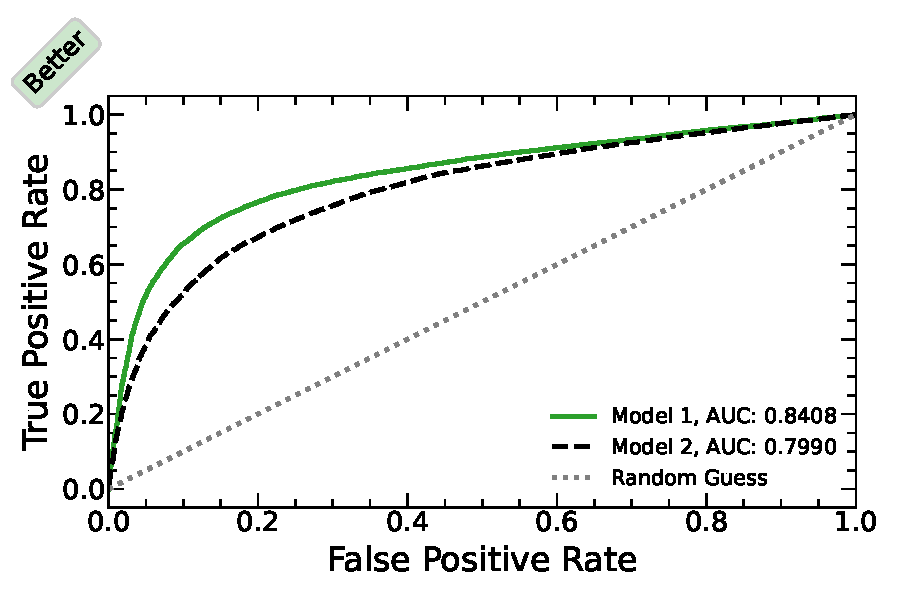
\includegraphics[width=\textwidth,trim={0.18cm 0.3cm 0.18cm 0.3cm},clip]{figures/ml/roc_curves/roc_model_1_model_2}% trim={<left> <lower> <right> <upper>}
  \caption{TPR versus FPR}
  \label{fig:ml:roc:standard}
  \end{subfigure}
  ~
  \begin{subfigure}[c]{0.48\textwidth}\centering
  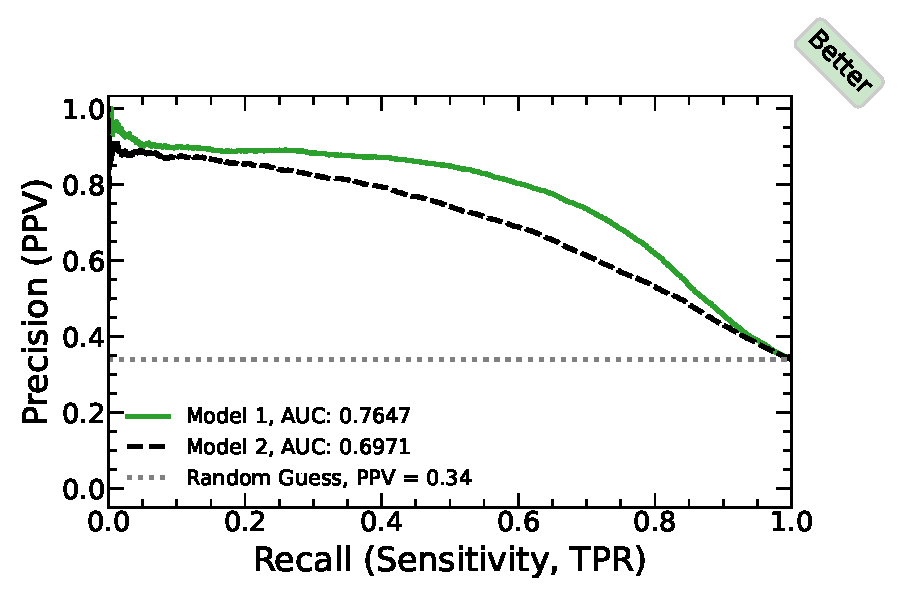
\includegraphics[width=\textwidth,trim={0.18cm 0.3cm 0.18cm 0.3cm},clip]{figures/ml/roc_curves/roc_precision_recall_model_1_model_2}% trim={<left> <lower> <right> <upper>}
  \caption{Precision versus Recall}
  \label{fig:ml:roc:precision_recall}
  \end{subfigure}
\caption{
Example ROC and precision-recall curves, generated \href{https://github.com/mepland/data_science_notes/blob/main/plots/plots.ipynb}{here}.
Note that model $1$ in solid green outperforms model $2$ when looking at both TPR versus FPR and precision versus recall.
The random guess line in the precision-recall plot is set by the class balance,
in this case the training set contained \SI{34}{\percent} positive examples.
}
\label{fig:ml:roc}
\end{figure}

\begin{figure}
  \centering
  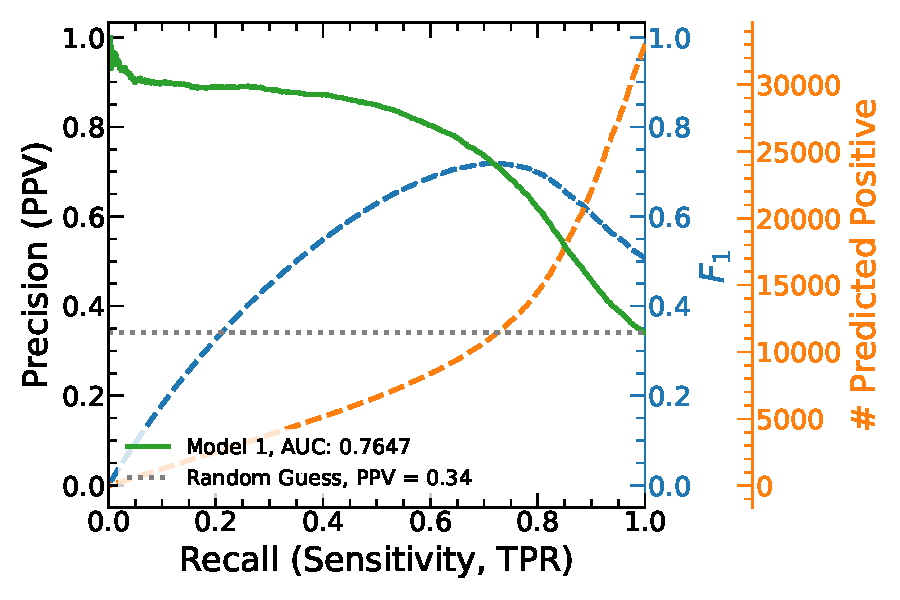
\includegraphics[width=0.7\textwidth,trim={0.18cm 0.3cm 0.18cm 0.3cm}]{figures/ml/roc_curves/roc_precision_recall_model_1_f1_n_pos}% trim={<left> <lower> <right> <upper>}
\caption{
Additional information, such as the $F_{1}$ score and number of predicted positives,
can be plotted as a function of recall on a single precision-recall plot,
at the cost of potentially making it harder to read.
}
\label{fig:ml:roc:precision_recall:extended}
\end{figure}

%%%%%%%%%%%%%%%%%%%%%%%%%%%%%%%%%%%%%%%%%%%%%%%%%%%%%%%%
\subsection{Concordance Statistic}
\label{ml_general:eval:concordance}

The concordance statistic, or $C$-statistic, \cref{eq:concordance:C} is a measure of goodness of fit
for binary classification and regression models, in particular being commonly used in survival analysis.
To begin we pick two observations at random from the $m$ available observations;
if the ordering of model's predicted \yhat values agrees\footnote{The treatment of ties depends on implementation,
see \href{https://cran.r-project.org/web/packages/survival/vignettes/concordance.pdf}{here}
for the survival analysis concordance function in \R.} with the order of the true $y$ values,
then the pair of observations is said to be concordant\footnote{In survival analysis,
we take a random pair of subjects and their lifetime predictions.
If the subject the model predicted to have a longer lifetime
did in fact have the longer observed lifetime, the pair is concordant.}.
By measuring the fraction of concordant pairs over all pairs we arrive at the concordance statistic.

\begin{subequations} \label{eq:concordance}
\begin{align}
C &= \frac{1}{ \binom{m}{2} } \sum_{i \neq j} \text{Concordance}\left(i, j\right), \label{eq:concordance:C} \\
&= \text{ROC AUC} = \int_{0}^{1} \text{TPR}\, \dd{\left(\text{FPR}\right)}, \label{eq:concordance:ROC_AUC} \\
&= P\left(\yhat_{i} < \yhat_{j} \mid y_{i} < y_{j} \right), \label{eq:concordance:P} \\
\text{Concordance}\left(i, j\right) &= \begin{dcases}
1 & \yhat_{i} < \yhat_{j},\, y_{i} < y_{j}, \\
0 & \yhat_{i} \geq \yhat_{j},\, y_{i} < y_{j}.
\end{dcases} \label{eq:concordance:concordance} \\
\end{align}
\end{subequations}

The concordance statistic ranges from $0$ to $1$,
with $0.5$ being equivalent to random guessing and $1$ representing ideal performance.
The ROC AUC\footnote{The ROC curve should have TPR on the vertical axis and FPR on the horizontal axis as in \cref{fig:ml:roc:standard}.} and $C$-statistic are equivalent for
binary classification\footnote{The model must be setup such that the $y=1$ class receives the higher \yhat prediction.},
both representing the probability that
the model will rank a randomly chosen $y=1$ observation above a randomly chosen $y=0$ observation \cite{Hand2001,Fawcett2006861}.

%%%%%%%%%%%%%%%%%%%%%%%%%%%%%%%%%%%%%%%%%%%%%%%%%%%%%%%%
\subsection{Impact of Class Priors}
\label{ml_general:eval:class_priors}

The true ratio of positive and negative classes in a dataset
will affect the above performance metrics,
making fair comparisons across datasets difficult;
particularly when working with data that has a class imbalance, see \cref{class:imbalance}.
One approach for handling these situations is to calibrate the metrics
at a reference class ratio before comparison,
as explained in \cite{1909.02827}.

%%%%%%%%%%%%%%%%%%%%%%%%%%%%%%%%%%%%%%%%%%%%%%%%%%%%%%%%
\subsection{Multi-Class Extensions}
\label{ml_general:eval:multi_class}
% TODO Multi-Class ROC AUC extensions \cite{Hand2001}

%%%%%%%%%%%%%%%%%%%%%%%%%%%%%%%%%%%%%%%%%%%%%%%%%%%%%%%%
\subsection{Akaike Information Criterion (AIC)}
\label{ml_general:eval:AIC}

The Akaike information criterion (AIC) \cite{1100705}
is a metric for comparing the performance of multiple models,
balancing their raw performance against their complexity.
It was derived from information theory underpinnings by Akaike,
and estimates the information lost, \ie underfitting,
by a model when compared to the true model, \ie reality.
The performance of the model is captured in a
log-likelihood term, $\log\left(\hat{L}\right)$,
where $\hat{L}$ is the maximum value of the model's likelihood function.
The model's complexity is incorporated via $k$, the number of parameters in the model\footnote{Including parameters of the assumed errors,
\eg \iid normal errors with a mean of 0 would still contribute 1 parameter from the unknown variance, per dimension.}.
The AIC is then:

\begin{equation} \label{eq:AIC}
\text{AIC} = 2k - 2\log\left(\hat{L}\right).
\end{equation}

When computing the AIC for multiple models,
the best performing model will tend to have the lowest AIC.
Note that AIC is a relative measure;
a low AIC does not guarantee good absolute model performance.
Differences in AIC can be interpreted via the relative likelihood,
$\exp\left(\left(\text{AIC}_{\text{min}} - \text{AIC}_{i}\right)/2\right)$,
which is proportional to the probability that model $i$ minimizes the information loss.
For example, $\exp\left(\left(100 - 110\right)/2\right) = \num{0.007}$ implies that
a model with $\text{AIC} = 110$ is only $\num{0.007}$ times as probable
to minimize the information loss as a $\text{AIC}_{\text{min}} = 100$ model.

The AIC is only asymptotically valid,
and model specific $\order{k^{2}}$ corrections may be needed
if the training set size $n$ is small compared to $k$.
For example, the AIC with corrections (AICc) for a linear,
univariate model with normally distributed residuals, \ie linear regression, is:

\begin{equation} \label{eq:AICc}
\text{AICc} = \text{AIC} + \frac{2k^{2}+2k}{n-k-1}.
\end{equation}

Lastly, as the AIC compares multiple statistical models in a general way,
it can be used as a theoretical basis for hypothesis testing, and statistics in general,
grounded in information theory rather than the frequentist or Bayesian frameworks.

%%%%%%%%%%%%%%%%%%%%%%%%%%%%%%%%%%%%%%%%%%%%%%%%%%%%%%%%
\subsection{Bayesian Information Criterion (BIC)}
\label{ml_general:eval:BIC}
The Bayesian information criterion (BIC) \cite{10.1214/aos/1176344136}
is very similar to the AIC, but derived within the Bayesian framework.
It assumes a uniform prior\footnote{The AIC can be derived from a different prior \cite{doi:10.1177/0049124104268644},
but can also be formulated independently of any Bayesian framework.} over the models being considered,
leading to a larger model complexity term \cite{1311138} of
$k\ln\left(n\right)$, where $n$ is the size of training set:

\begin{equation} \label{eq:BIC}
\text{BIC} = k\ln\left(n\right) - 2\log\left(\hat{L}\right).
\end{equation}

Again, the BIC is both a relative measure of performance,
with lower BIC values being better,
and an approximate measure, valid when $k \ll n$.
When a model's residuals are independent and identically distributed (\iid) normal random variables,
and $\pdv*{\log\left(\hat{L}\right)}{\left(\text{true variance}\right)} = 0$,
the BIC simplifies \cite{priestley1981spectral} to

\begin{subequations} \label{eq:BIC_gaus_errors}
\begin{align}
\text{BIC} &= k\ln\left(n\right) + n \ln\left(\hat{\sigma}_{e}^{2}\right) + C\left(n\right), \label{eq:BIC_gaus_errors:BIC} \\
\hat{\sigma}_{e}^{2} &= \frac{1}{n} \sum_{i=1}^{n} \left(x_{i} - \hat{x}_{i}\right)^{2} = \frac{1}{n} \text{RSS}, \label{eq:BIC_gaus_errors:RSS}
\end{align}
\end{subequations}

\noindent where RSS is the residual sum of squares,
commonly used in ordinary least squares (OLS) regression,
and $C\left(n\right)$ is a function of $n$ alone\footnote{This term
likely absorbs the error's variance parameter from where it should appear in $k$.}, independent of the model.

\subsubsection{AIC and BIC Comparisons}
\label{ml_general:eval:BIC_comp_AIC}

In the limit $n \to \infty$ the BIC is guaranteed to select the true model,
if the true model is in the set of models under consideration,
which is not guaranteed with the AIC.
However, we commonly do not have the true model in our set of possible models,
and $n$ may be small in comparison to $k$.
In these cases, the AIC can select a better model than BIC
\cite{1311138,doi:10.1177/0049124104268644,Vrieze_2012,8498082}.
In practice these differences do not have a large impact;
as both the AIC and BIC are readily provided by statistical software
they can both be used to pick a few leading models
for a final comparison on absolute performance.

%%%%%%%%%%%%%%%%%%%%%%%%%%%%%%%%%%%%%%%%%%%%%%%%%%%%%%%%
%%%%%%%%%%%%%%%%%%%%%%%%%%%%%%%%%%%%%%%%%%%%%%%%%%%%%%%%
\section{Model Calibration}
\label{ml_general:calibration}

Many classification models return \yhat values between \num{0} and \num{1}
which can be interpreted as the predicted probability $\hat{p} = P\left(y=1 \mid \vb{x}\right)$.
However, some model types, in particular
support vector machines (SVM) of \cref{class:SVM},
boosted models of \cref{ml_general:boosting},
and \naive Bayes models of \cref{class:naive_bayes},
have a tendency to produce distorted probability distributions\footnote{See
the caption of \cref{fig:ml_general:calibration_curves} for
a description of the miscalibration tendencies of these models.
Essentially, all three model types listed here will experience
sigmoidal distortions in their calibration curves,
which is the reason for the effectiveness of Platt scaling.},
as shown by a non-linear calibration curve.
This is not an issue if we only need the ordinality of the predictions,
\eg who are the top \SI{10}{\percent} patients at risk,
but must be addressed if we want to use \yhat as an actual probability,
or use a metric such as log loss, see \cref{ml_general:loss_func:log_loss},
or the ROC curve\footnote{ROC curves, and thus ROC AUC,
can be affected by miscalibration as they are created by measuring the performance of the model
as the classification threshold is varied between \num{0} and \num{1}.
If the model is miscalibrated this can lead to an uneven sampling of the model's performance,
and thus a distorted ROC curve.},
see \cref{ml_general:eval:ROC}, which depend on the probability.
Methods for calibrating\footnote{Regression models can also be calibrated \cite{10.1093/aje/154.9.836,1806.07690},
but are omitted here.} a model's output such that
predictions of $\yhat = \hat{p}$ actually have $\hat{p} = P\left(y=1 \mid \vb{x}\right)$
include\footnote{Other calibration methods include Bayesian binning into quantiles \cite{pmid25927013},
and histogram binning \cite{10.5555/645530.655658}.} Platt scaling,
isotonic regression,
and beta calibration\footnote{The beta calibration paper \cite{beta_calib}
is also a great review of Platt scaling and isotonic regression,
and includes a hypothesis test for calibration.} \cite{10.1145/1102351.1102430,1706.04599,beta_calib,2112.10327}.

When calibrating a classifier it is highly recommended to use cross validation
to separate the data used for model training and calibration.
\sklearn provides a convenient \texttt{CalibratedClassifierCV}
\href{https://scikit-learn.org/stable/modules/generated/sklearn.calibration.CalibratedClassifierCV.html}{class}
to implement Platt and isotonic calibration with cross validation.

%%%%%%%%%%%%%%%%%%%%%%%%%%%%%%%%%%%%%%%%%%%%%%%%%%%%%%%%
\subsection{Calibration Curves}
\label{ml_general:calibration:calibration_curves}

We can visualize the degree of a model's miscalibration with a calibration curve,
also known as a reliability diagram,
by plotting the observed fraction of true positives $p_{0}$ against
the uncalibrated predicted fraction of positives $\hat{p}_{u}$,
see \cref{fig:ml_general:calibration_curves} for examples.
The points of the curve are created by taking
the mean $p_{0}$ of data points binned in $\hat{p}_{u}$,
typically either uniformly or by quantiles\footnote{Using quantiles,
\ie each bin has the same number of events, is recommended.}.
Deviation from the straight line $p_{0} = \hat{p}_{u}$ are evidence of miscalibration.
As a reminder, it is vital to construct
the calibration curve with a set of data distinct from the training set.

\begin{figure}[H]
  \centering
  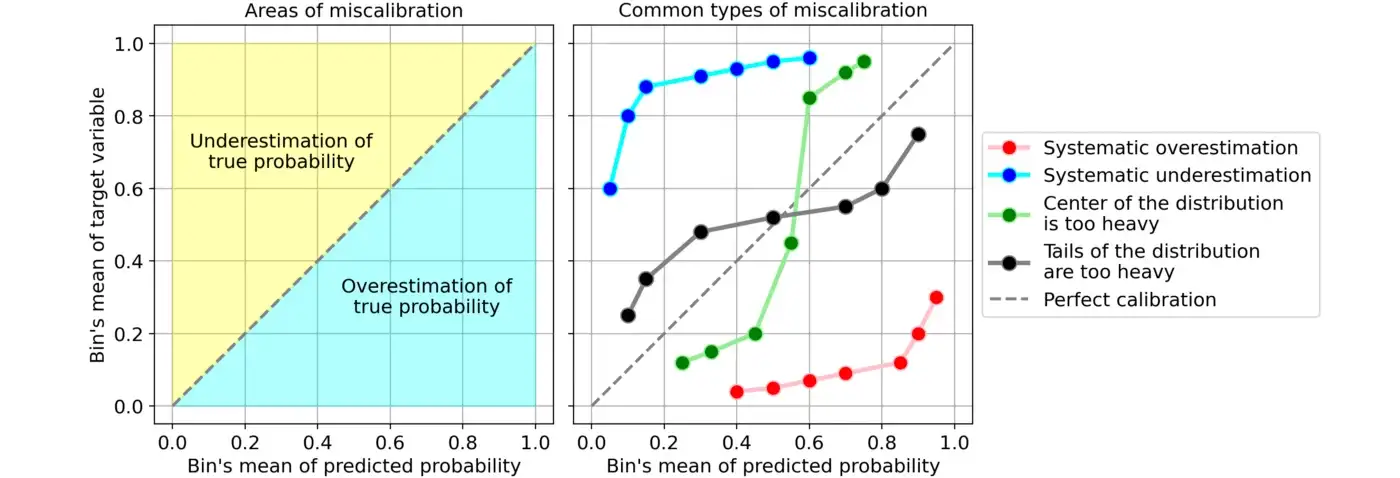
\includegraphics[width=\textwidth]{figures/ml/miscalibration_illustration.png}
\caption{
Example calibration curves for common types of miscalibration,
from \href{https://towardsdatascience.com/pythons-predict-proba-doesn-t-actually-predict-probabilities-and-how-to-fix-it-f582c21d63fc}{Samuele Mazzanti}.
SVM, and other maximum margin methods, as well as boosted trees tend to push \yhat away from \num{0} and \num{1},
see the green `center' curve;
while \naive Bayes models tend to push \yhat toward \num{0} and \num{1} \cite{10.1145/1102351.1102430},
see the black `tails' curve.
If a classifier is trained on an unbalanced dataset biased toward negative examples,
the uncalibrated \yhat may be systemically biased toward \num{1},
see the red `overestimation' curve.
}
\label{fig:ml_general:calibration_curves}
\end{figure}

%%%%%%%%%%%%%%%%%%%%%%%%%%%%%%%%%%%%%%%%%%%%%%%%%%%%%%%%
\subsection{Calibration Metrics}
\label{ml_general:calibration:calibration_metrics}

We can quantify the degree of a classifiers calibration with the
expected calibration error (ECE) and Brier score.

\subsubsection{Expected Calibration Error (ECE)}
\label{ml_general:calibration:ECE}

The expected calibration error (ECE) \cite{pmid25927013} \cref{eq:calibration:ECE}
is a weighted mean of the calibration error
across the bins of the calibration curve.
Note that $y=0,1$, $0 \leq \yhat \leq 1$,
and that in $\expval{y}, \expval{\yhat}$ we are taking the mean over all points in bin $b$.
The choice of binning can affect the ECE,
see \href{https://towardsdatascience.com/pythons-predict-proba-doesn-t-actually-predict-probabilities-and-how-to-fix-it-f582c21d63fc}{here} for
more details and a \python implementation\footnote{ECE is also implemented in
the \textsc{TorchMetrics}, \href{https://torchmetrics.readthedocs.io/en/stable/classification/calibration_error.html}{documentation},
\textsc{TensorFlow}, \href{https://www.tensorflow.org/probability/api_docs/python/tfp/stats/expected_calibration_error}{documentation},
libraries.}.

\begin{equation} \label{eq:calibration:ECE}
\text{ECE} = \frac{1}{m} \sum_{b \,\in\, \text{bins}} \abs{\expval{y} - \expval{\yhat}}_{b} \, m_{b} \, .
\end{equation}

\subsubsection{Brier score}
\label{ml_general:calibration:brier_score}

The Brier score\footnote{Named after the original author \cite{brier},
though that formulation is slightly different and can handle multi-class settings.} \cref{eq:calibration:brier} is
similar to the ECE, but takes the difference per data point $i$.
It is equivalent to the mean squared error (MSE) of the probabilities.
\sklearn has a convenient \texttt{brier\_score\_loss}
\href{https://scikit-learn.org/stable/modules/generated/sklearn.metrics.brier_score_loss.html}{function}.

\begin{equation} \label{eq:calibration:brier}
\text{Brier} = \frac{1}{m} \sum_{i=1}^{m} \left(y_{i} - \yhat_{i}\right)^{2}.
\end{equation}

%%%%%%%%%%%%%%%%%%%%%%%%%%%%%%%%%%%%%%%%%%%%%%%%%%%%%%%%
\subsection{Platt Scaling}
\label{ml_general:calibration:platt}

One of the simplest methods of calibrating
an uncalibrated classifier $\yhat_{u}$ is Platt scaling \cite{platt_scaling},
where a logistic regression model, \cref{class:logistic},
is fit on $\mb{X} = \yhat_{u}$ to predict the true $y = 0, 1$.
Essentially, the logistic regression model will scale $\yhat_{u}$ as

\begin{equation} \label{eq:calibration:platt}
\hat{p} = P\left(y=1 \mid \vb{x}\right) = \frac{1}{1+\exp\left(-\gamma\left(\yhat_{u} - m\right)\right)}\,,
\end{equation}

\noindent where $\gamma \geq 0$, $m$ are the fitted scaling
parameters\footnote{Here we have used the parameterization from \cite{beta_calib},
which highlights that $m$ controls where the midpoint $\hat{p}=\num{0.5}$ appears in $\yhat_{u}$,
while $\gamma$ is a shape parameter that controls the curves slope.
$\gamma \geq 0$ is required to make the curve monotonically non-decreasing.}. However,
instead of training the logistic regression model to predict $y = 0, 1$ directly,
Platt scaling applies a Bayesian correction\footnote{See \cite{platt_scaling} for a full explanation,
but basically this correction arises by assuming the out-of-sample data
has a finite possibility of having the opposite label than the in-sample data.
Note that $t \to y$, $t_{+} \to 1$ and $t_{-} \to 0$, as $N \to \infty$.} to
predict $t_{+}$, $t_{-}$ instead:

\begin{equation} \label{eq:calibration:platt_t}
\begin{gathered}
t_{+} = \frac{N_{+}+1}{N_{+}+2} \enspace \text{for} \enspace y = 1, \\
t_{-}= \frac{1}{N_{-}+2} \enspace \text{for} \enspace y = 0.
\end{gathered}
\end{equation}

Platt scaling does well when the calibration error is symmetrical \cite{10.1145/1102351.1102430}
and can be corrected via a sigmoid transformation.
This has been empirically shown \cite{platt_scaling} for
support vector machines\footnote{Platt scaling
is even baked in to the \sklearn
\href{https://scikit-learn.org/stable/modules/svm.html\#scores-and-probabilities}{SVM implementation}.} (SVM), \cref{class:SVM},
but is not true in general.

If $\gamma = 1$, $m = 0$ \cref{eq:calibration:platt} becomes the
inverse logit function\footnote{Implemented in \scipy as the
\texttt{expit} \href{https://docs.scipy.org/doc/scipy/reference/generated/scipy.special.expit.html}{function}.},
also known as the sigmoid function,
which is a useful function\footnote{\xgboost, \cref{fig:small_example_CART}
and \figs, \cref{class:FIGS}, use this trick.} for quickly scaling a model's internal scores to
sensible values between \num{0} and \num{1},
although \yhat is still uncalibrated in this case.

%%%%%%%%%%%%%%%%%%%%%%%%%%%%%%%%%%%%%%%%%%%%%%%%%%%%%%%%
\subsection{Isotonic Regression}
\label{ml_general:calibration:isotonic_regression}

Isotonic regression \cite{isotonic_calib} is a non-parametric calibration method
that only assumes the required correction has the form of a monotonically non-decreasing, \ie isotonic, step function,
unlike Platt scaling which assumes the form is a sigmoid function.
Isotonic regression can thus better fit calibration curves,
particularity when the miscalibration is non-symmetric,
provided there is enough\footnote{An empirical guideline is $\num{1000} < N$ \cite{10.1145/1102351.1102430}.
For $N < \num{1000}$ beta calibration is a better choice.} data to avoid overfitting.
The non-parametric piecewise curve is fit by minimizing

\begin{equation} \label{eq:calibration:isotonic_regression}
L = \sum_{i}^{N} \left(y_{i} - \yhat_{i,\,c} \right)^{2},
\end{equation}

\noindent where $\yhat_{i,\,c} \leq \yhat_{j,\,c}$
whenever $\yhat_{i,\,u} \leq \yhat_{j,\,u}$.

%%%%%%%%%%%%%%%%%%%%%%%%%%%%%%%%%%%%%%%%%%%%%%%%%%%%%%%%
\subsection{Beta Calibration}
\label{ml_general:calibration:beta_calib}

Beta calibration \cite{beta_calib} is a newer parameterized method developed
to address shortcomings in the Platt scaling approach.
The name comes from the initial assumption that
the classifier's scores follow a beta distribution for each class\footnote{Really,
it is a slightly weaker assumption that
that the ratio of positive and negative score distributions
follows the ratio of two beta distributions.},
but the crucial improvement is the addition of a second shape parameter \cref{eq:calibration:beta},
for a total of 3 parameters\footnote{Note,
we require \cref{eq:calibration:beta} to be monotonically non-decreasing $\implies 0 \leq a,b$.} versus Platt's 2.
See \cite{beta_calib} for full details, but essentially this second shape parameter
allows us to drop homoscedasticity assumption
between the positive and negative class score variances
which is inherent in Platt scaling.

\begin{equation} \label{eq:calibration:beta}
\hat{p} = P\left(y=1 \mid \vb{x}\right) = \frac{1}{1+1/\left(e^{c} \frac{\yhat_{u}^{a}}{\left(1-\yhat_{u}\right)^{b}}\right)}\,.
\end{equation}

The increased parameterization of the beta calibration allows for
the identity function\footnote{This is also the basis for the hypothesis test for calibration \cite{beta_calib}.},
when $a=b=1$, $c=0$, thereby leaving already calibrated models alone\footnote{This allows
beta calibration to be integrated into automatic ML pipelines without as many safety checks.},
unlike Platt scaling which would always introduce some distortions.
See \cref{fig:calibration:beta_examples:beta_calib_naive_bayes} for an example of this effect.
With $1<a=b$, we regain a sigmoid-like calibration similar to Platt,
as well as an inverse sigmoid-like calibration with $a=b<1$.
See \cref{fig:calibration:beta_curves} for an illustration of the possible beta calibration curves.

\begin{figure}[H]
  \centering
  \begin{subfigure}[b]{0.48\textwidth}\centering
    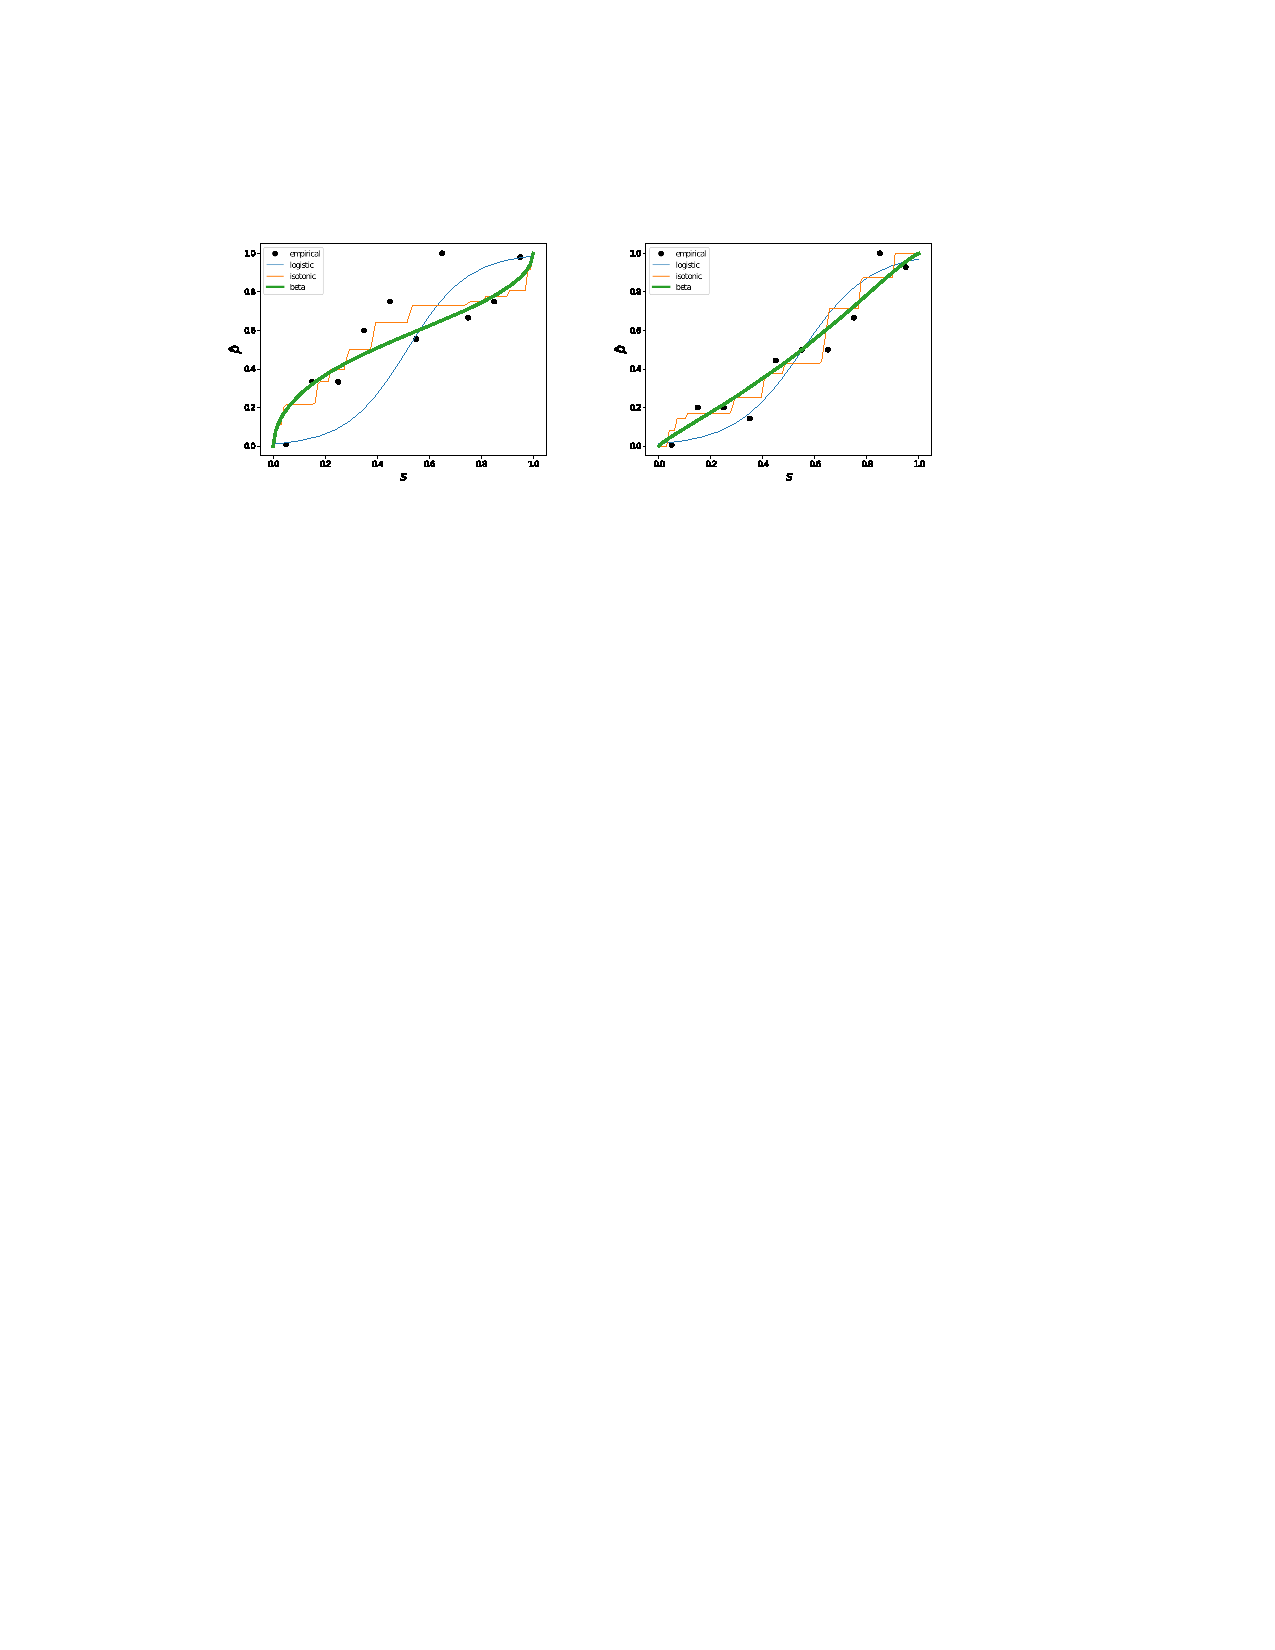
\includegraphics[height=5.8cm,trim={0cm 0cm 6.5cm 0cm},clip]{figures/ml/beta_calib_examples}% trim={<left> <lower> <right> <upper>}
  \caption{AdaBoost}
  \label{fig:calibration:beta_examples:beta_calib_adaboost}
  \end{subfigure}
  ~
  \begin{subfigure}[b]{0.48\textwidth}\centering
    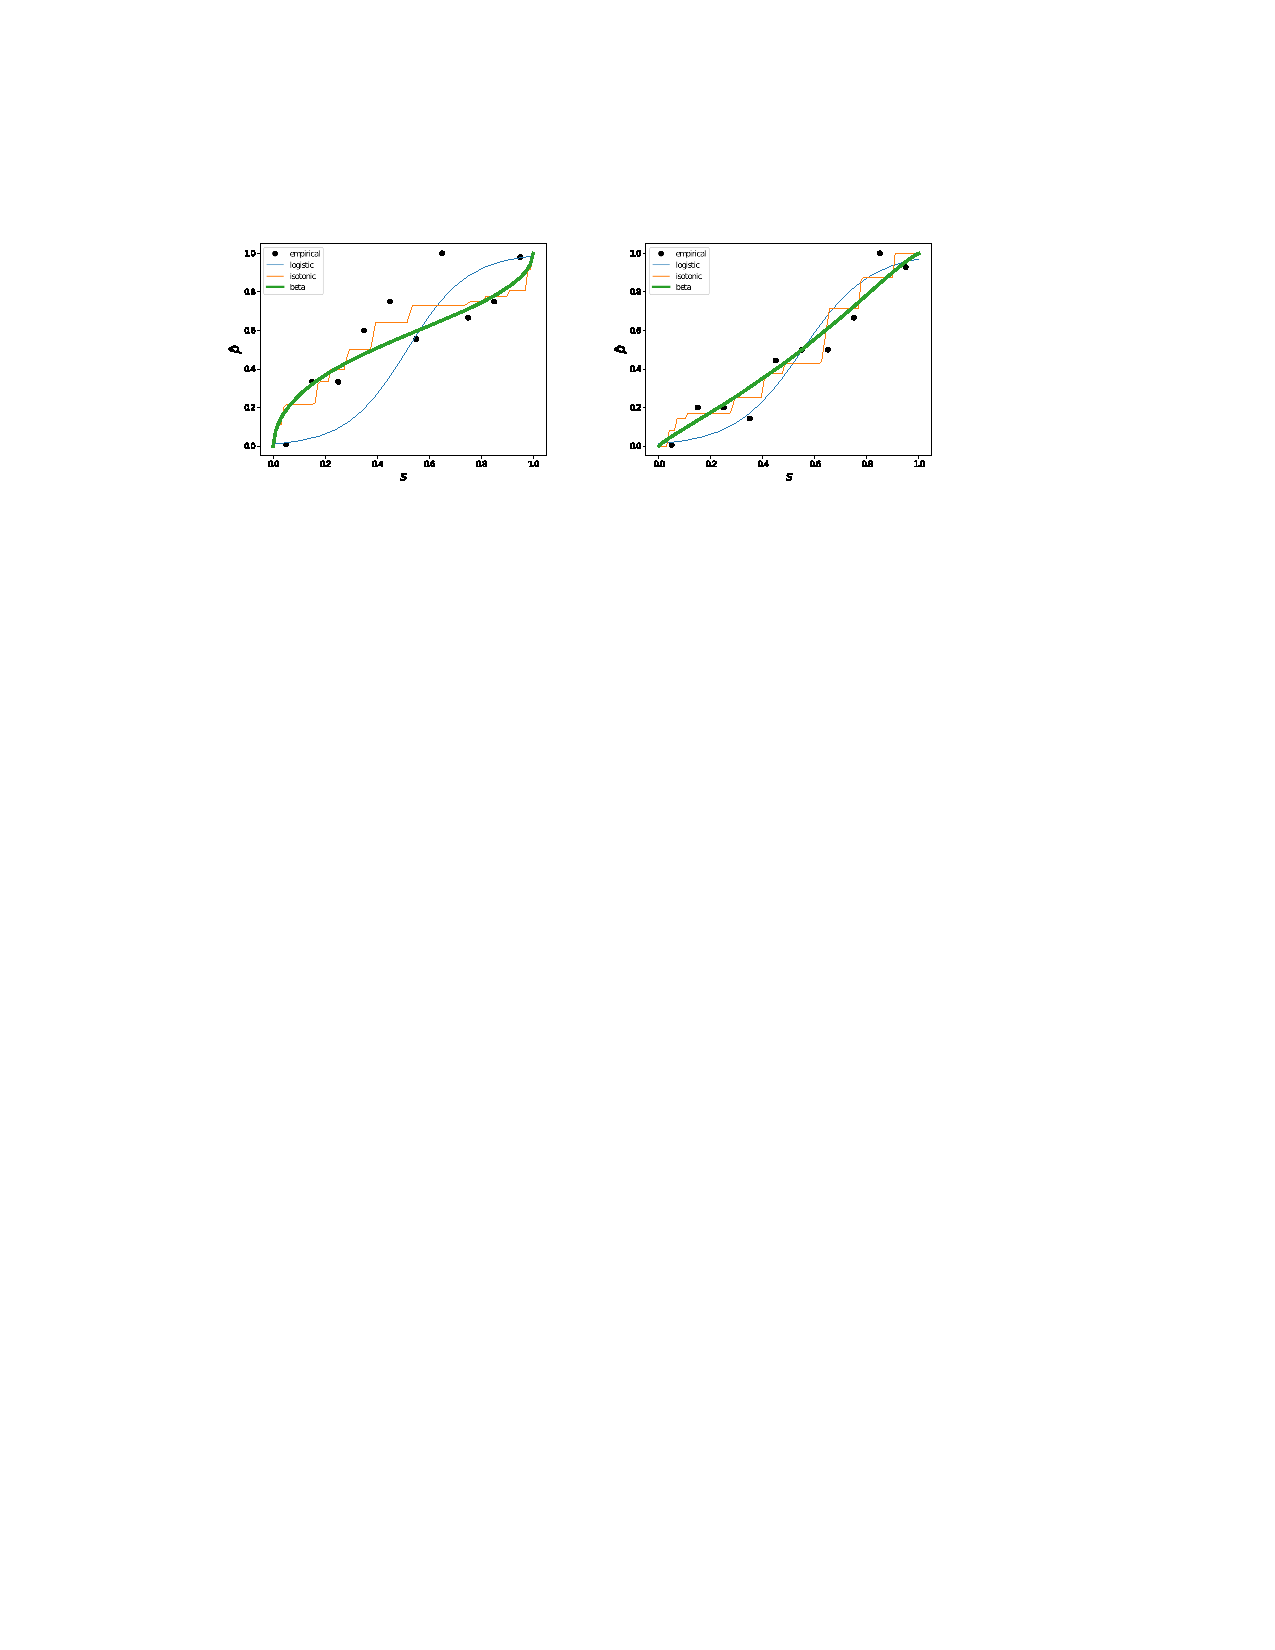
\includegraphics[height=5.8cm,trim={6.5cm 0cm 0cm 0cm},clip]{figures/ml/beta_calib_examples}% trim={<left> <lower> <right> <upper>}
  \caption{\Naive Bayes}
  \label{fig:calibration:beta_examples:beta_calib_naive_bayes}
  \end{subfigure}
\caption{
A comparison of Platt, \ie logistic, isotonic, and beta calibration
methods for two classification models \cite{beta_calib}.
Here $s = \yhat_{u}$ is the uncalibrated score.
In both examples Platt scaling actually makes things worse,
while beta calibration outperforms isotonic calibration.
Note that in \cref{fig:calibration:beta_examples:beta_calib_naive_bayes}
the classifier is almost fully calibrated to start,
in which case beta calibration does not disturb the scores,
unlike Platt scaling.
\label{fig:calibration:beta_examples}
}
\end{figure}

\begin{figure}[H]
  \centering
  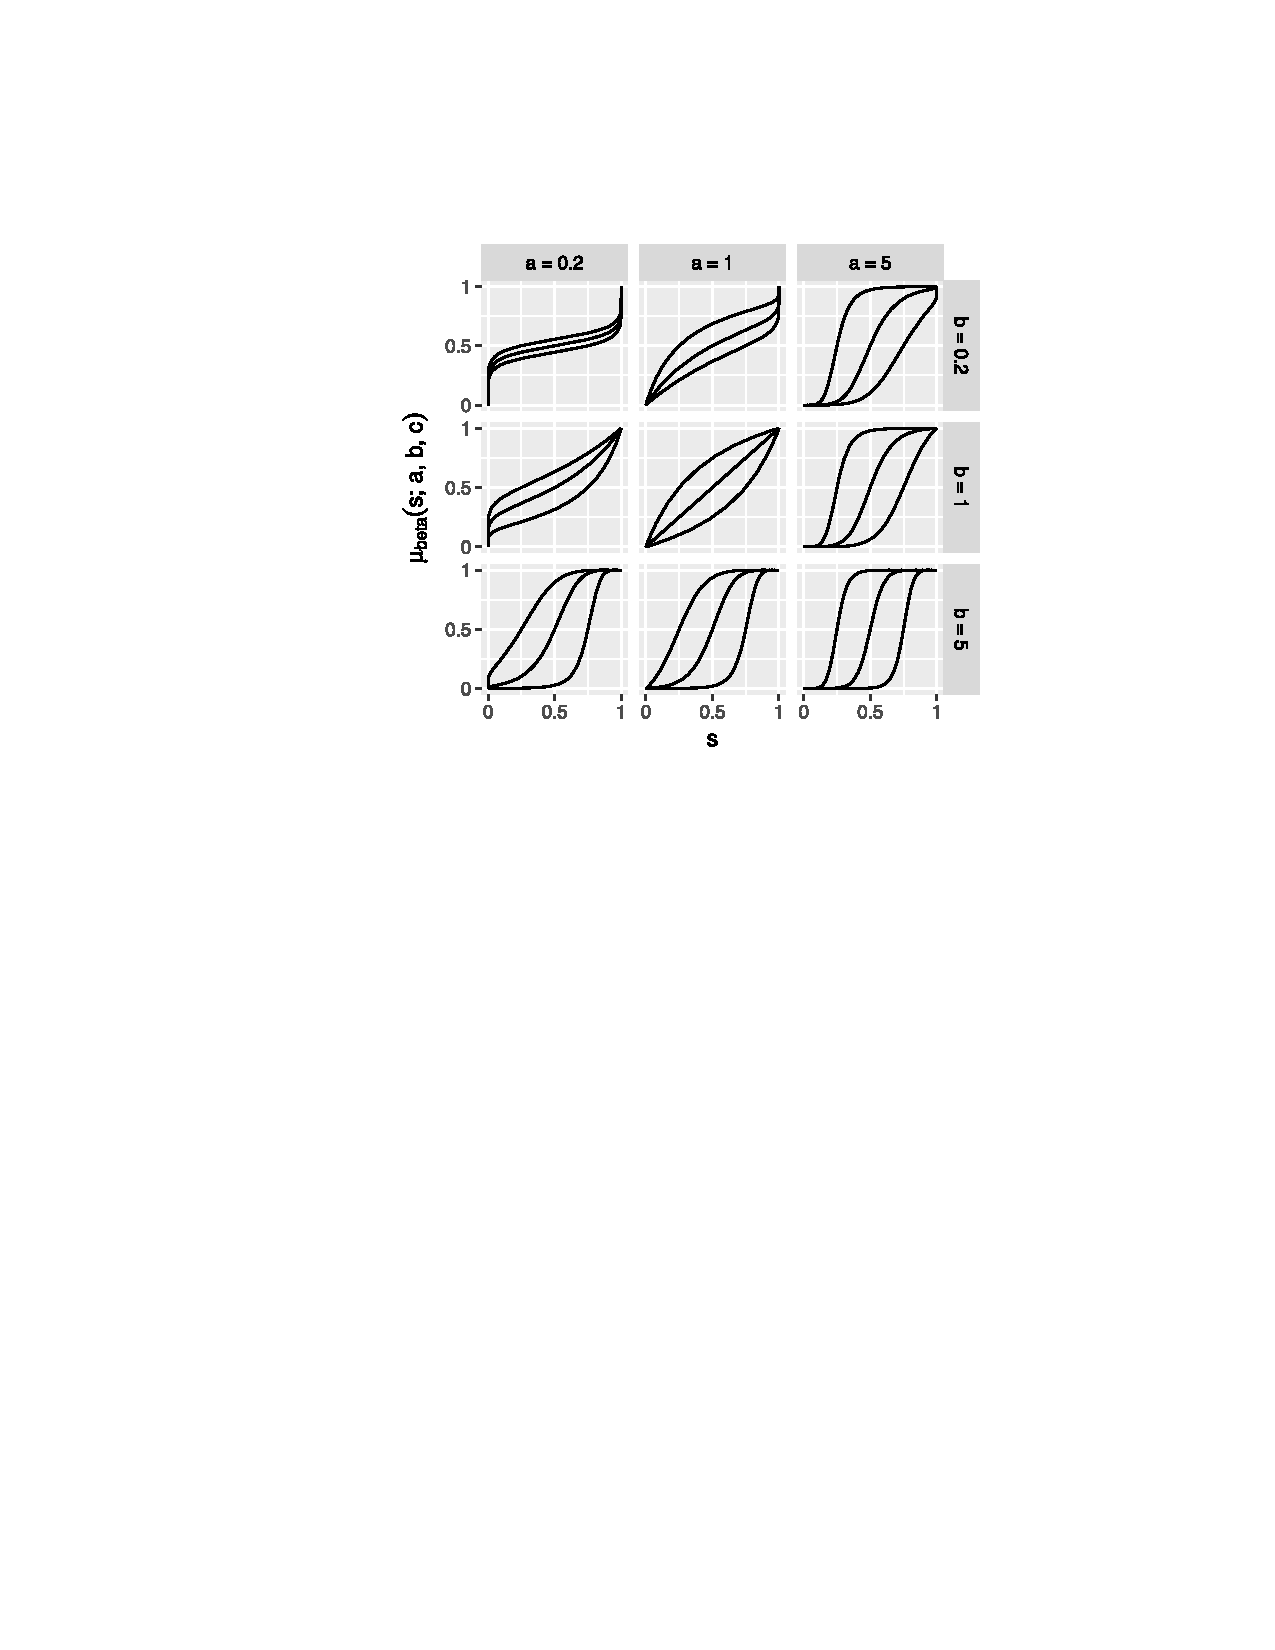
\includegraphics[width=0.6\textwidth]{figures/ml/beta_calib_curves}
\caption{
Example beta calibration curves with
$a, b \in \{0.2, 1, 5\}$,
and $c = b \ln\left(1 - m\right) - a\ln\left(m\right)$
where $m \in \{0.25, 0.5, 0.75\}$ \cite{beta_calib}.
Note the identity function in the center where $a=b=1$, $c=0$,
sigmoid-like (inverse sigmoid-like) curves in the bottom right (top left) corner
where $1<a=b$ ($a=b<1$),
and asymmetric curves where $a \neq b$.
}
\label{fig:calibration:beta_curves}
\end{figure}

\python and \R implementations for beta calibration
are provided by the original authors in the \texttt{betacal} \href{https://betacal.github.io/}{package}.
The authors have also developed a multiclass extension \cite{10.5555/3454287.3455390}.
Lastly, according to the empirical studies of \cite{beta_calib},
beta calibration generally does better than logistic calibration,
and outperforms isotonic calibration on smaller datasets.

%%%%%%%%%%%%%%%%%%%%%%%%%%%%%%%%%%%%%%%%%%%%%%%%%%%%%%%%
%%%%%%%%%%%%%%%%%%%%%%%%%%%%%%%%%%%%%%%%%%%%%%%%%%%%%%%%
\section{Selecting a Decision Threshold}
\label{ml_general:decision_threshold}

% include \cref to significance section, if eventually added

In physics we may try to maximize the significance $Z$ of a classifier\footnote{In practice,
particle physicists work with the \href{https://en.wikipedia.org/wiki/Neyman\%E2\%80\%93Pearson\_lemma}{Neyman-Pearson framework}
to construct likelihood-ratio based tests specific to an analysis, and then optimize that significance.} by
picking an optimal point along the ROC or precision-recall curve to set the decision threshold.
However in data science it is often better to create a payoff matrix of the anticipated
benefits associated with a TP or TN, and costs associated with a FP or FN,
for the particular business case at hand.
The expected value of any decision threshold can quickly be computed
from the payoff matrix elements, $\expvalE{\hat{A} \mid B}$, as

\begin{equation} \label{eq:E_profit}
\expvalE{\text{profit}} = \sum_{A,B} \expvalE{\hat{A} \mid B} P\left(\hat{A} \mid B \right) P\left(B\right),
\end{equation}

\noindent where $A$ and $B$ are any two cases.
The optimal decision threshold can then be found by maximizing $\expvalE{\text{profit}}$.

%%%%%%%%%%%%%%%%%%%%%%%%%%%%%%%%%%%%%%%%%%%%%%%%%%%%%%%%
%%%%%%%%%%%%%%%%%%%%%%%%%%%%%%%%%%%%%%%%%%%%%%%%%%%%%%%%
\section{Bias-Variance Tradeoff}
\label{ml_general:bias_variance_tradeoff}

\begin{enumerate}[noitemsep]
  \item Bias: Errors due to a model not learning about relationships between features in the training data, \ie underfitting. Caused by invalid relationships present in the model.
  \item Variance: Errors due to an overly complex model failing to generalize beyond the training data, \ie overfitting. Caused by sensitivity to small fluctuations in the training data.
\end{enumerate}

\begin{figure}[H]
  \centering
  \savebox{\largestimage}{
    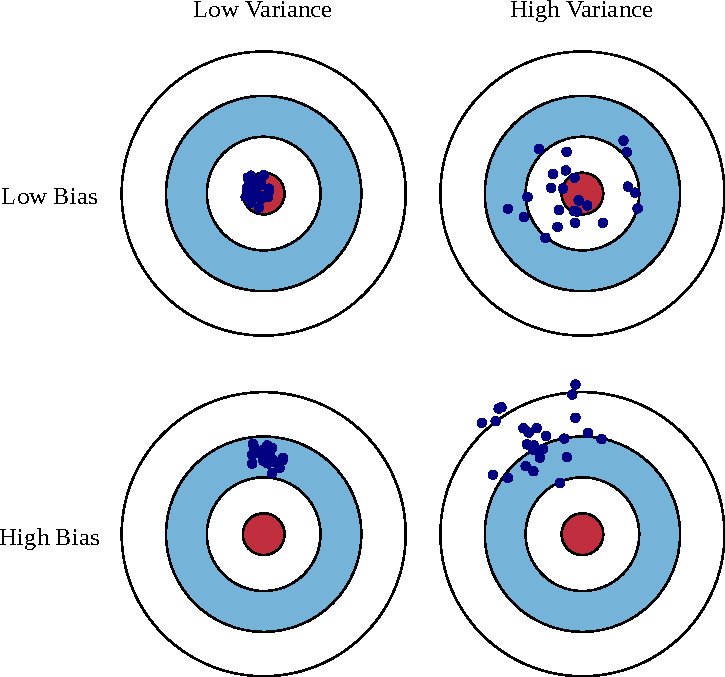
\includegraphics[width=0.47\textwidth]{figures/ml/bias_variance_tradeoff}
  }% Store largest image in a box

  \begin{subfigure}[b]{0.48\textwidth}\centering
    \usebox{\largestimage}
    \vspace{0.01cm}
  \caption{Direct Comparison}
  \label{fig:ml:bias_variance_tradeoff:direct}
  \end{subfigure}
  ~
  \begin{subfigure}[b]{\wd\largestimage}\centering
    \raisebox{\dimexpr.5\ht\largestimage-.5\height}{% Adjust vertical height of smaller image
      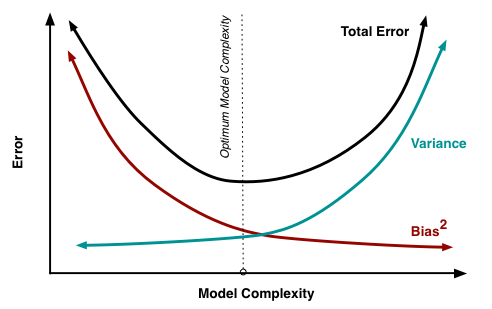
\includegraphics[width=\textwidth]{figures/ml/bias_variance_error_tradeoff.png}}
  \caption{Error Components (Test Set)}
  \label{fig:ml:bias_variance_tradeoff:error}
  \end{subfigure}
\caption{
Illustrations of the bias-variance tradeoff,
by \href{http://scott.fortmann-roe.com/docs/BiasVariance.html}{Scott Fortmann-Roe}.
\label{fig:ml:bias_variance_tradeoff}
}
\end{figure}

Every model makes a tradeoff between bias and variance,
which is roughly controlled by its level of complexity
as can be seen in \cref{fig:ml:bias_variance_tradeoff:error}.
\Cref{fig:ml_general:early_stopping} shows this in practice,
as past a certain point of complexity the validation error grows
while the training error continues to decrease.

\subsubsection{Mean Square Error (MSE) Decomposition}
\label{ml_general:bias_variance_tradeoff:decop}

We can analytically decompose the mean square error (MSE) into explicit
bias, variance, and irreducible error components\footnote{See
\cite{pmlr-v151-shuo-tan22a} for a similar decomposition for decision trees.}.
Let $y = f\left(\vb{x}\right) + \epsilon$ represent
the observed data, $y_{i}$, $\vb{x}_{i}$,
where $f\left(\vb{x}\right)$ is the true parent distribution\footnote{$\expval{f} = f$ is deterministic,
and acts as a constant as far as expectation values are concerned.} and
$\epsilon$ is random noise\footnote{This is the source of the irreducible error.
Since future data will still have $\epsilon$, the predictions can't be perfect
-- even when neglecting the model's own bias and variance.}\footnote{Later we'll need
$\sigma^{2} = \variance{\epsilon} = \expval{\epsilon^{2}} - \expval{\epsilon}^{2} = \expval{\epsilon^{2}}$.} having
$\expval{\epsilon} = 0$, $\variance{\epsilon} = \sigma^{2}$.
Representing the trained model\footnote{Note
that $\cov{\epsilon}{\hat{f}} = 0 \implies \expval{\epsilon \hat{f}} = \expval{\epsilon} \expval{\hat{f}}$.} as
$\hat{f}\left(\vb{x}\right)$, we expand the MSE:

\begin{subequations} \label{eq:bias_variance_tradeoff:decop}
\begin{align}
\text{MSE} &= \expval{\left(y-\hat{f}\right)^{2}}\,, \\
&= \expval{\left(f + \epsilon - \hat{f} + \big[\expval{\hat{f}}-\expval{\hat{f}}\big]\right)^{2}}\,, \\
&= \expval{\left(\big[f - \expval{\hat{f}}\big] + \epsilon - \big[\hat{f} - \expval{\hat{f}}\big]\right)^{2}}\,, \\
&= \expval{\left(f-\expval{\hat{f}}\right)^{2}}
+\expval{\epsilon^{2}}
+\expval{\left(\hat{f}-\expval{\hat{f}}\right)^{2}}
+2\expval{\left(f-\expval{\hat{f}}\right)\epsilon} \\
&\hphantom{=}-2\expval{\epsilon\left(\hat{f}-\expval{\hat{f}}\right)}
-2\expval{\left(f-\expval{\hat{f}}\right)\left(\hat{f}-\expval{\hat{f}}\right)}\,, \\
&= \left(-1\right)^{2}\left(\expval{\hat{f}}-f\right)^{2} +\sigma^{2} + \variance{\hat{f}}
+2\left(f-\expval{\hat{f}}\right)\cancelto{0}{\expval{\epsilon}} \\
&\hphantom{=}-2\cancelto{0}{\expval{\epsilon}}\left(\expval{\hat{f}}-\expval{\hat{f}}\right)
-2\left(f-\expval{\hat{f}}\right)\cancelto{0}{\left(\expval{\hat{f}}-\expval{\hat{f}}\right)}\,, \\
&= \left(\bias{\hat{f}}\right)^{2} + \variance{\hat{f}} + \sigma^{2}\,.
\end{align}
\end{subequations}

%%%%%%%%%%%%%%%%%%%%%%%%%%%%%%%%%%%%%%%%%%%%%%%%%%%%%%%%
%%%%%%%%%%%%%%%%%%%%%%%%%%%%%%%%%%%%%%%%%%%%%%%%%%%%%%%%
\section{Bootstrap Aggregation, \texorpdfstring{\ie}{ie} Bagging}
\label{ml_general:bagging}

Bootstrap aggregation, more commonly known as bagging\footnote{As in
\textbf{b}ootstrap \textbf{agg}regat\textbf{ing},
and the bags of data utilized by the method.} \cite{Breiman1996},
is an application of bootstrapping, see \cref{stats:bootstrapping}, to machine learning.
When bagging, we construct an ensemble model from multiple component models,
each trained in parallel on a different bootstrapped sample of the training dataset.
The outputs of the component models are then aggregated into one ensemble result,
taking the mode predicted class (mean value) when working with classification (regression) models.
\cref{fig:bagging_and_boosting:bagging} provides an overview of the method,
while Random Forests, described in \cref{class:RF}, are one implementation.
By repeatedly sampling the training data we reduce the chance of overfitting,
and thus bagging is one method of lowering a model's variance
at the cost of increased computation in training and inference.

\begin{figure}[H]
\centering
  \begin{subfigure}[c]{0.48\textwidth}\centering
  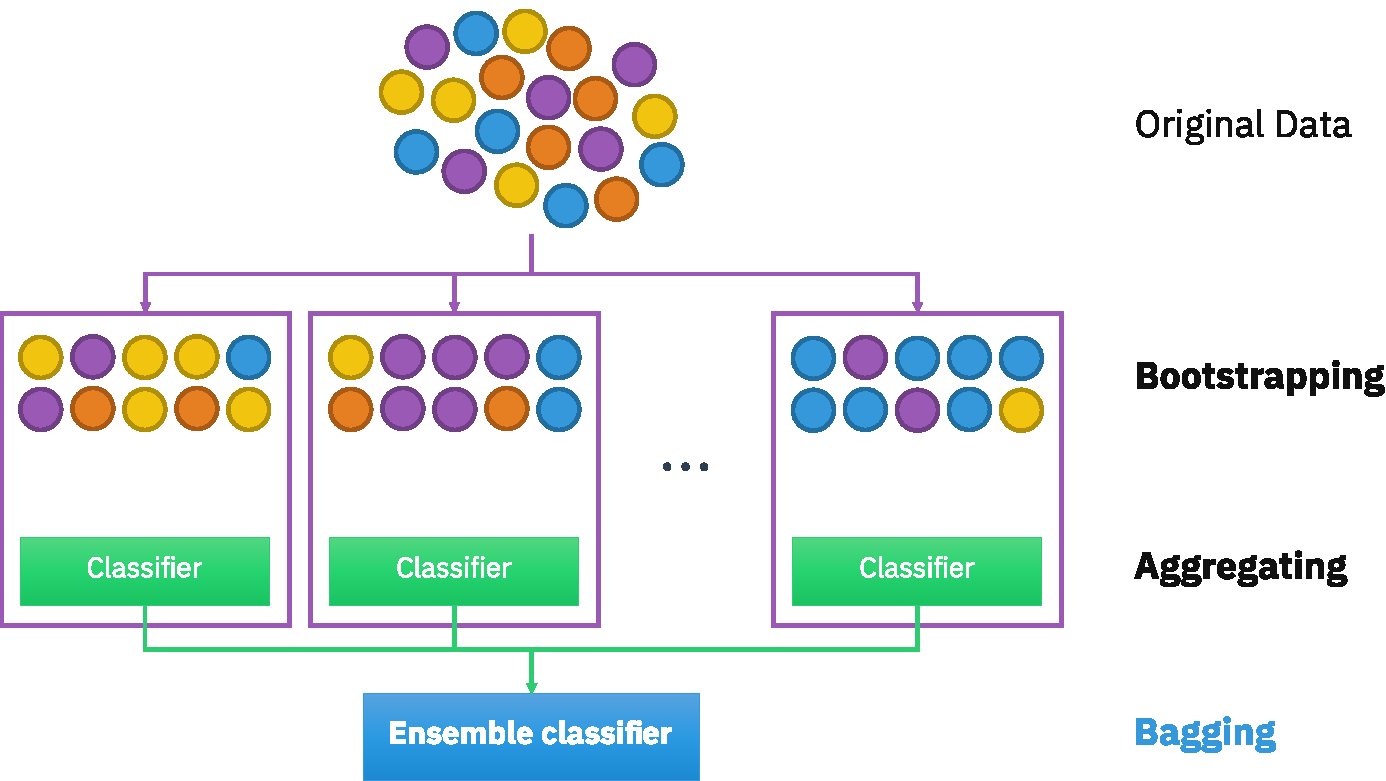
\includegraphics[width=\textwidth]{figures/ml/bagging}
  \vspace{0.1cm}
  \caption{Bagging}
  \label{fig:bagging_and_boosting:bagging}
  \end{subfigure}
  \quad
  \begin{subfigure}[c]{0.48\textwidth}\centering
  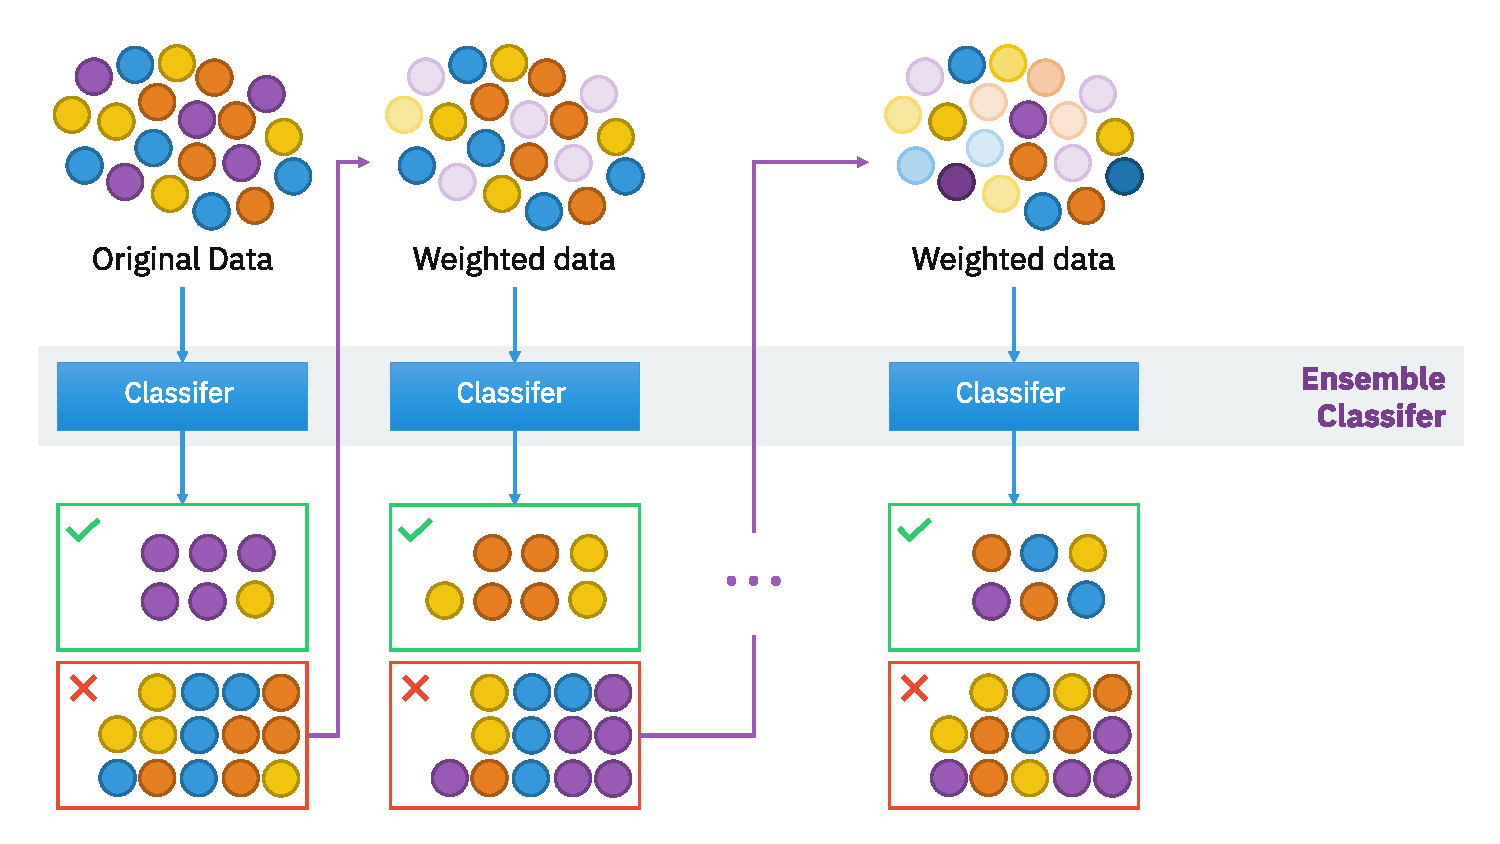
\includegraphics[width=\textwidth]{figures/ml/boosting}
  \vspace{0.1cm}
  \caption{Boosting}
  \label{fig:bagging_and_boosting:boosting}
  \end{subfigure}
\caption{
Illustrations of the bagging and boosting ensemble methods,
by \href{https://en.wikipedia.org/wiki/File:Ensemble_Bagging.svg}{Sirakorn}
and \href{https://en.wikipedia.org/wiki/File:Ensemble_Boosting.svg}{Sirakorn}.
Note that bagging tends to reduce variance,
while boosting can reduce bias and variance.
}
\label{fig:bagging_and_boosting}
\end{figure}
%%%%%%%%%%%%%%%%%%%%%%%%%%%%%%%%%%%%%%%%%%%%%%%%%%%%%%%%
%%%%%%%%%%%%%%%%%%%%%%%%%%%%%%%%%%%%%%%%%%%%%%%%%%%%%%%%
\section{Boosting}
\label{ml_general:boosting}

Boosting \cite{10.5555/3091696.3091715,FREUND1997119,Breiman1996BiasV,friedman2000}
is an ensemble method similar in concept to bagging.
However instead of simply taking multiple random bootstrap samples in parallel,
when boosting we train a series of models iteratively,
as shown in \cref{fig:bagging_and_boosting:boosting}.
At each iteration $i$, data points poorly predicted
by the ensemble of the previous $i-1$ models are upsampled\footnote{In practice,
this can be done with a literal upsampling of points in the training set,
or by the application of training weights,
provided model and software library support them.} giving them
greater weight when computing the loss function for model $i$.
In this way, we can create an ensemble model with a lower bias than any of
the component models\footnote{Boosting thus works best when applied to high bias, low variance component models,
while bagging works best for low bias, high variance models.
Note that in either case the component models are typically decision trees,
but in general can be a heterogeneous mix of different model types.},
while also reducing variance\footnote{The adaptive resampling component of the boosting algorithm
can lead to a reduction in variance in much the same way as the resampling performed in bagging \cite{Breiman1996BiasV}.
Note that the term arcing, \ie \textbf{a}daptive \textbf{r}esampling and \textbf{c}ombin\textbf{ing}, used in \cite{Breiman1996BiasV}
is an early name for boosting.}.
A prime example of boosting's ability to improve the performance weak models via ensembling
can be seen in Boosted Decision Trees (BDT) as described in \cref{class:BDT}.

%%%%%%%%%%%%%%%%%%%%%%%%%%%%%%%%%%%%%%%%%%%%%%%%%%%%%%%%
%%%%%%%%%%%%%%%%%%%%%%%%%%%%%%%%%%%%%%%%%%%%%%%%%%%%%%%%
\section{Model Interpretability}
\label{ml_general:interp}
% TODO

%%%%%%%%%%%%%%%%%%%%%%%%%%%%%%%%%%%%%%%%%%%%%%%%%%%%%%%%
\subsection{Feature Importance}
\label{ml_general:interp:feature_importance}
% TODO

%%%%%%%%%%%%%%%%%%%%%%%%%%%%%%%%%%%%%%%%%%%%%%%%%%%%%%%%
%%%%%%%%%%%%%%%%%%%%%%%%%%%%%%%%%%%%%%%%%%%%%%%%%%%%%%%%
\section{Regularization}
\label{ml_general:reg}

Regularization is a method for controlling the variance (overfitting)
of a model by putting constraints on the size of its parameters.
In terms of \cref{ml_general:bias_variance_tradeoff}, regularization forces the model's
bias to grow on the training set in order to lower the variance on future data.
The two main types of regularization are shown in \cref{eq:L1_L2}
and depend on different powers of the norm\footnote{In
the case of OLS linear regression the constant intercept term $\beta_{0}$ is not included in $\norm{\vb*{\beta}}$.} of the model parameters $\vb*{\beta}$.
In order to treat all features equally, normalization must be used before applying regularization.
A hyperparameter $\lambda$ is included to tune the amount of regularization applied in the objective function,
$S\left(\vb*{\beta}\right) = L + \Omega$.
As $\lambda$ is increased, it decreases the size the model's coefficients, and thereby its variance (overfitting),
up to a point when the model is unable to adequately train on the available data and the bias (underfitting) begins to grow.

\begin{subequations} \label{eq:L1_L2}
\begin{align}
\Omega_{\text{L1}}\left(\vb*{\beta}\right) &= \lambda \norm{\vb*{\beta}}\hphantom{^{1}}
= \lambda \sum_{j=1}^{n} \, \abs{\beta_{j}}\,, \label{eq:L1} \\
\Omega_{\text{L2}}\left(\vb*{\beta}\right) &= \lambda \norm{\vb*{\beta}}^{2}
= \lambda \sum_{j=1}^{n} \,\, \beta_{j}^{2}\,. \label{eq:L2}
\end{align}
\end{subequations}

For a particular value of $\lambda$, the effect of L1 and L2 regularization\footnote{Here
$q$ is being used as the power of $\norm{\vb*{\beta}}$. For L1 (L2), $q=1$ ($q=2$).} is
to constrain $\norm{\vb*{\beta}}^{q} \leq t\left(\lambda\right)$ for some $t\left(\lambda\right)$.
As can be seen in \cref{fig:ml:l1l2} the L1 norm constrains $\vb*{\beta}$ to lie within a hypercube,
while the L2 constraint is a hypersphere.

\begin{figure}[H]
  \centering
  \begin{subfigure}[b]{0.48\textwidth}\centering
      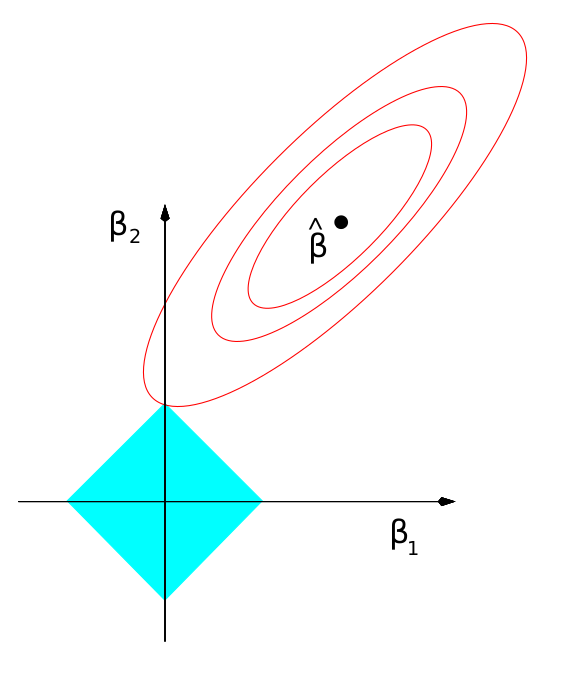
\includegraphics[width=\textwidth]{figures/ml/l1}
  \caption{L1}
  \label{fig:ml:l1l2:l1}
  \end{subfigure}
  ~
  \begin{subfigure}[b]{0.48\textwidth}\centering
      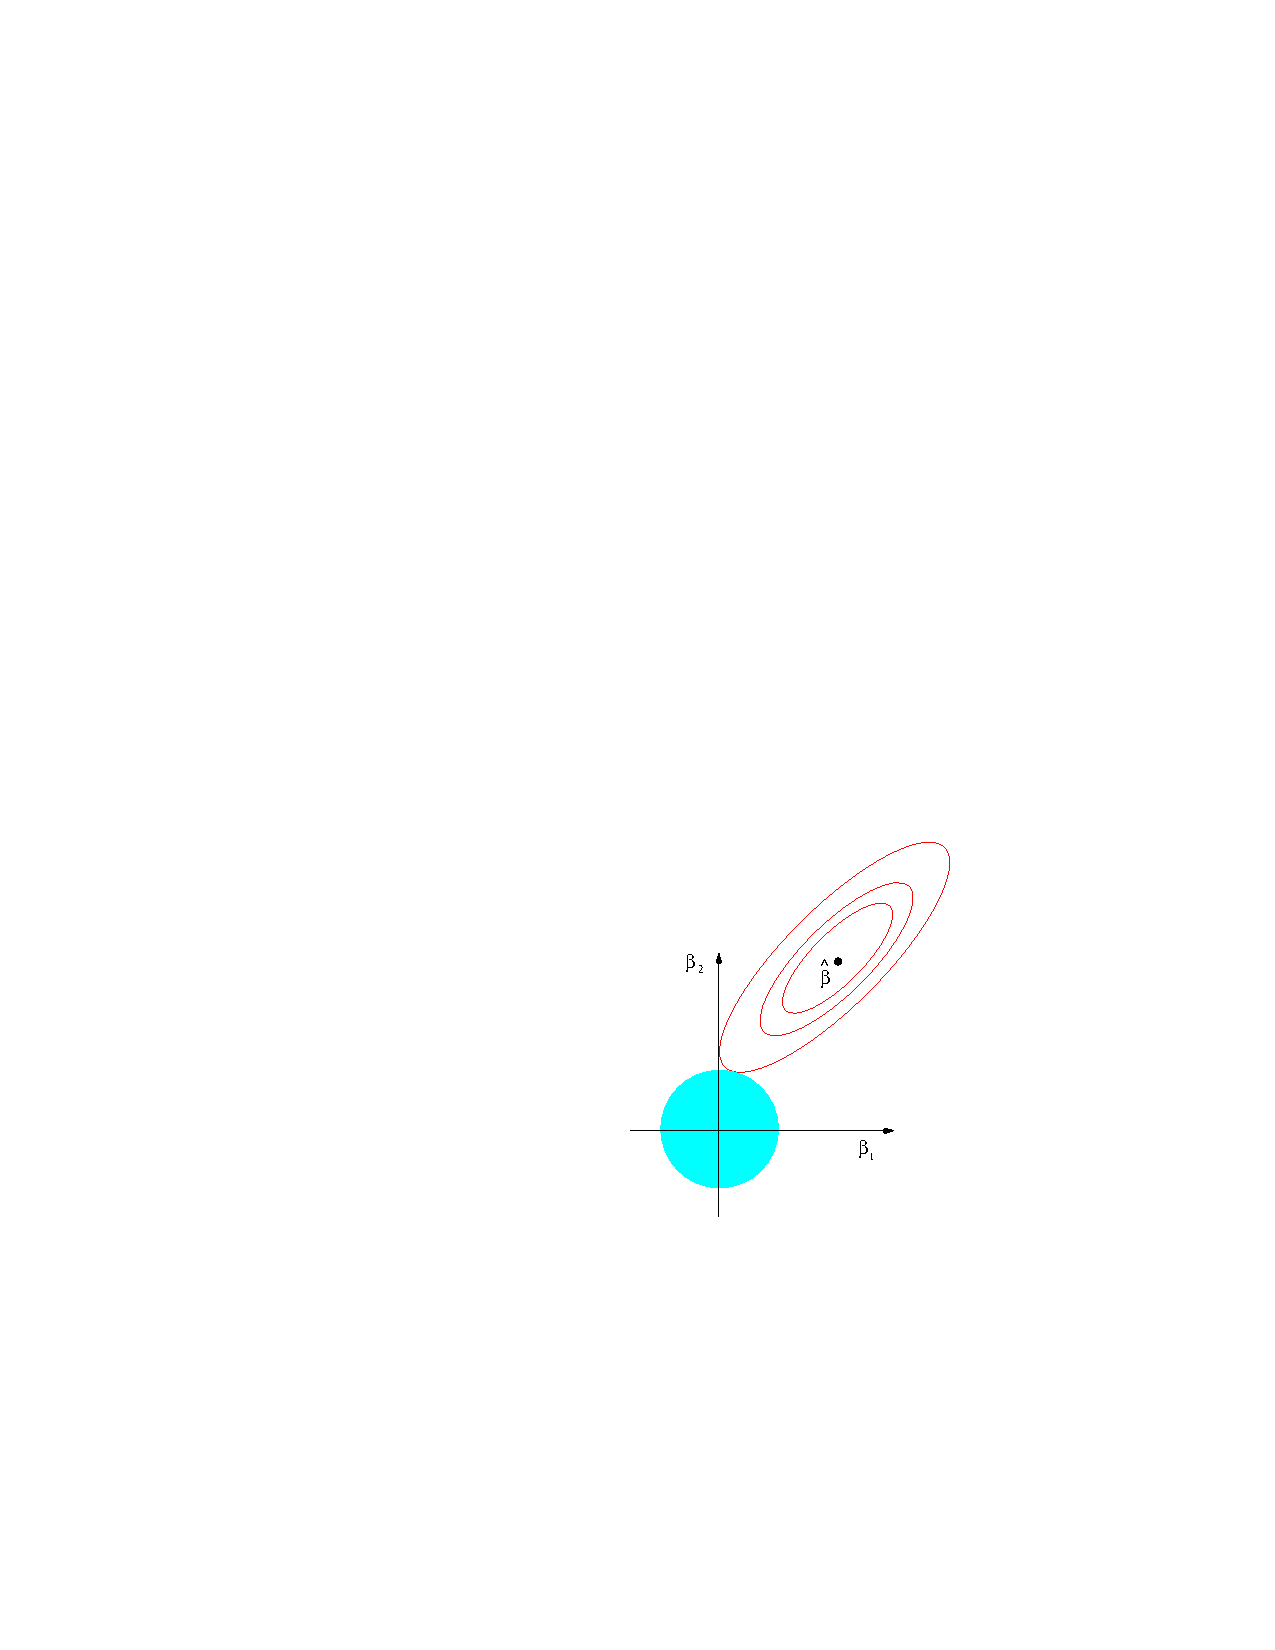
\includegraphics[width=\textwidth]{figures/ml/l2}
  \caption{L2}
  \label{fig:ml:l1l2:L2}
  \end{subfigure}
\caption{
A graphical representation of the L1 and L2 regularization constraints on $\vb*{\beta}$ \cite{HastieTF09}.
The best value of $\vb*{\beta}$ for optimizing the loss function $L$ is indicated as $\hat{\vb*{\beta}}$.
For a given contour in $L$, L1 will tend to force $\vb*{\beta}$ along one of the axes,
identically setting some $\beta_{i}$ coefficients to zero,
while L2 is rotationally symmetric and has no such tendencies.
\label{fig:ml:l1l2}
}
\end{figure}

%%%%%%%%%%%%%%%%%%%%%%%%%%%%%%%%%%%%%%%%%%%%%%%%%%%%%%%%
\subsection{L1 -- LASSO}
\label{ml_general:reg:L1}

L1, or LASSO\footnote{Least Absolute Shrinkage and Selection Operator.},
regularization uses the norm $\norm{\vb*{\beta}}$ \cref{eq:L1}, or taxi cab distance.
As its geometric constraints on $\vb*{\beta}$ are hypercubes,
it tends to set some model parameters to 0, creating sparsity,
and thereby acts as a form of built-in feature selection.

%%%%%%%%%%%%%%%%%%%%%%%%%%%%%%%%%%%%%%%%%%%%%%%%%%%%%%%%
\subsection{L2 -- Ridge}
\label{ml_general:reg:L2}

L2, or ridge, regularization \cref{eq:L2} uses the square of the norm, or euclidean distance.
Models made with L2 regularization are somewhat less interpretable than those made with L1,
as L2 may make many parameters very small, but does not remove them entirely.
The parameters are still shrunk toward zero, and each other,
while highly correlated features are effectively averaged.
L2 is slightly faster to run than L1 computationally as, unlike L1, it
is not represented as a piecewise function and has a closed form expression.

%%%%%%%%%%%%%%%%%%%%%%%%%%%%%%%%%%%%%%%%%%%%%%%%%%%%%%%%
\subsection{Elastic Net}
\label{ml_general:reg:EN}

L1 and L2 regularization can be used in combination
to take advantage of both of their benefits.
Such a combination is known as the elastic net penalty \cref{eq:elastic_net},
where the combination can be controlled via two $\lambda_{1}$, $\lambda_{2}$ hyperparameters,
or a shared $\lambda$ and mixing parameter $\alpha$.
Compared to LASSO, elastic net does better when given multiple highly correlated features
and is more stable, \ie less dependent on the particular training data.

\begin{equation} \label{eq:elastic_net}
\begin{split}
\Omega_{\text{EN}}\left(\vb*{\beta}\right) &= \lambda_{1} \norm{\vb*{\beta}} + \lambda_{2} \norm{\vb*{\beta}}^{2}\\
&= \lambda \left( \alpha\norm{\vb*{\beta}} + \left(1-\alpha\right)\norm{\vb*{\beta}}^{2} \right)
\end{split}
\end{equation}

% TODo connections to SVM (https://en.wikipedia.org/wiki/Elastic_net_regularization#Reduction_to_support_vector_machine)

%%%%%%%%%%%%%%%%%%%%%%%%%%%%%%%%%%%%%%%%%%%%%%%%%%%%%%%%
\subsection{Drop Out}
\label{ml_general:reg:Drop}
% TODO

%%%%%%%%%%%%%%%%%%%%%%%%%%%%%%%%%%%%%%%%%%%%%%%%%%%%%%%%
\subsection{Early Stopping}
\label{ml_general:reg:early_stopping}
% TODO
% TODO ref in text \cref{fig:ml_general:early_stopping}

\begin{figure}[H]
  \centering
  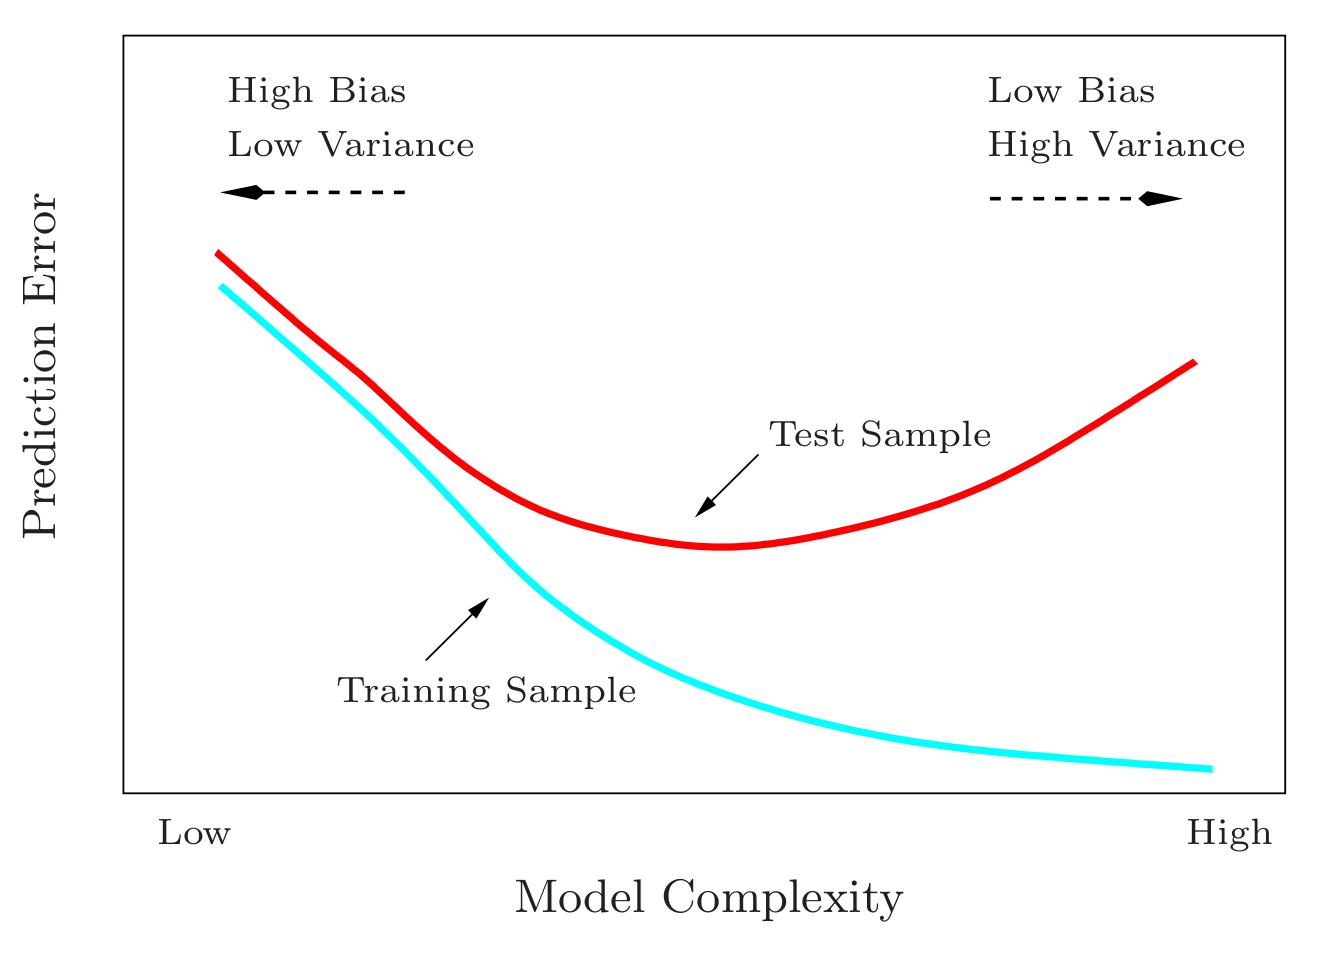
\includegraphics[width=0.8\textwidth]{figures/ml/test_train_err_curves}
\caption{
Illustrated effects of increasing model complexity on the error rates for the test and train sets \cite{HastieTF09}.
Early stopping would halt the training process when the test (or better yet, validation) set error stops decreasing.
This is also another example of the bias-variance tradeoff in action.
}
\label{fig:ml_general:early_stopping}
\end{figure}

%%%%%%%%%%%%%%%%%%%%%%%%%%%%%%%%%%%%%%%%%%%%%%%%%%%%%%%%
%%%%%%%%%%%%%%%%%%%%%%%%%%%%%%%%%%%%%%%%%%%%%%%%%%%%%%%%
\section{Selecting Training Set Size \texorpdfstring{$m$}{m}}
\label{ml_general:enough_training_data}
% TODO
% TODO ref in text \cref{fig:enough_training_data}

\begin{figure}
  \centering
  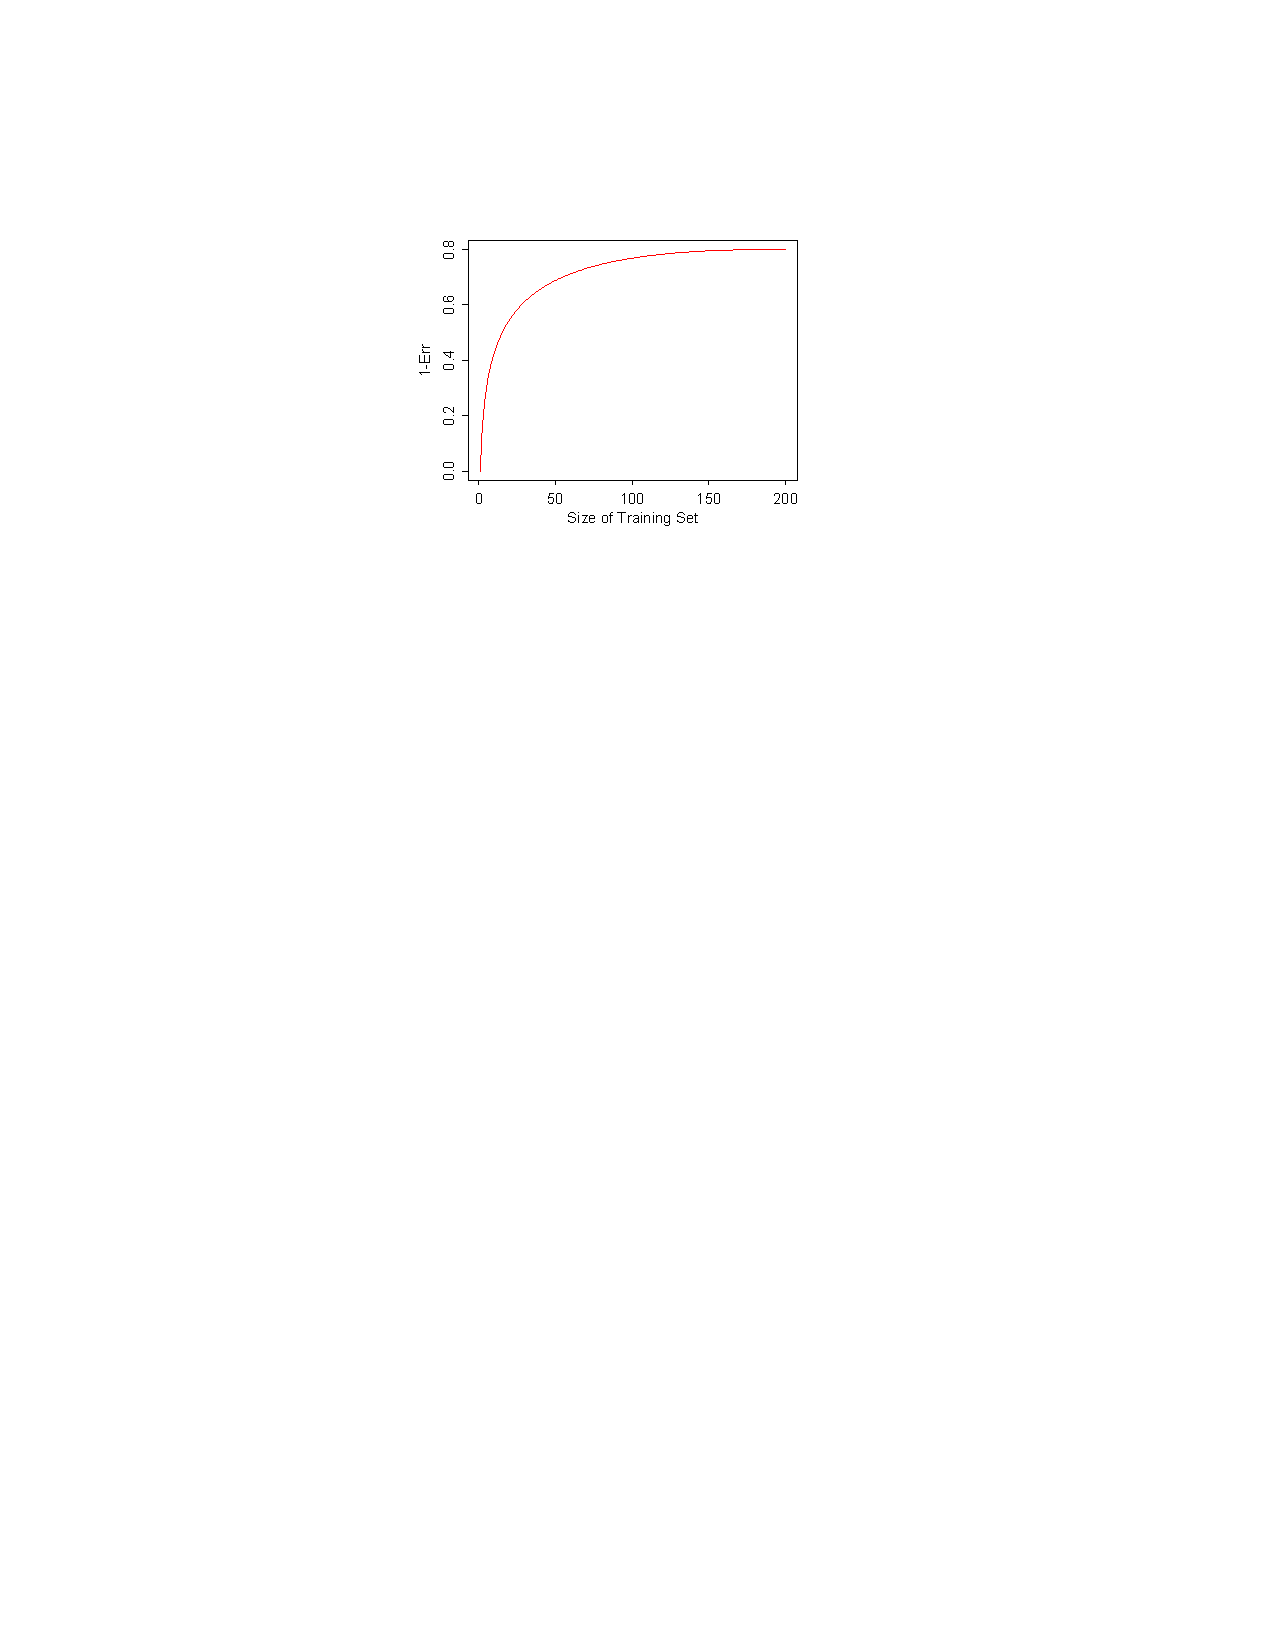
\includegraphics[width=0.8\textwidth]{figures/ml/acc_vs_m}
\caption{
Illustration of the decrease in classification error rate
with larger sets of training data \cite{HastieTF09}.
By artificially limiting the available number of data points $m$,
one can create a similar curve to verify that
there is enough statistics in the training data
for the complexity of the model under consideration.
Ideally the curve should reach a clear asymptote before the maximum $m$ is used.
}
\label{fig:enough_training_data}
\end{figure}

%%%%%%%%%%%%%%%%%%%%%%%%%%%%%%%%%%%%%%%%%%%%%%%%%%%%%%%%
%%%%%%%%%%%%%%%%%%%%%%%%%%%%%%%%%%%%%%%%%%%%%%%%%%%%%%%%
\section{Propensity Score Matching}
\label{ml_general:propensity}
% TODO

%%%%%%%%%%%%%%%%%%%%%%%%%%%%%%%%%%%%%%%%%%%%%%%%%%%%%%%%
%%%%%%%%%%%%%%%%%%%%%%%%%%%%%%%%%%%%%%%%%%%%%%%%%%%%%%%%
\section{Normalization}
\label{ml_general:normalization}
% TODO normalization of input features (for faster training, more equal regularization), batch renormalization in neural networks

%%%%%%%%%%%%%%%%%%%%%%%%%%%%%%%%%%%%%%%%%%%%%%%%%%%%%%%%
\subsection{Batch Renormalization}
\label{ml_general:reg:batch_renorm}
% TODO

%%%%%%%%%%%%%%%%%%%%%%%%%%%%%%%%%%%%%%%%%%%%%%%%%%%%%%%%
%%%%%%%%%%%%%%%%%%%%%%%%%%%%%%%%%%%%%%%%%%%%%%%%%%%%%%%%
\section{Loss Functions}
\label{ml_general:loss_func}

% TODO add more loss functions such as OLS / MSE

%%%%%%%%%%%%%%%%%%%%%%%%%%%%%%%%%%%%%%%%%%%%%%%%%%%%%%%%
\subsection{Log Loss}
\label{ml_general:loss_func:log_loss}

In two class, positive $y=1$ and negative $y=0$, classification problems
the log loss function is an appropriate choice of $L$:

\begin{equation} \label{eq:log_loss}
L = -\frac{1}{m} \sum_{j=1}^{m} \big(y_{j} \ln\left(\yhat_{j}\right) +\left(1-y_{j}\right) \ln\left(1-\yhat_{j}\right)\big).
\end{equation}

Log loss is also known as binary logistic loss,
cross-entropy loss, and binary cross-entropy loss.
Here $L$ is shown averaged over the $m$ examples,
but depending on the name and application this may not be the case.

% TODO \xgboost specific?
% L = \sum_{j=1}^{m} \left[y_{j} \ln\left(1 + \exp(-\yhat_{j})\right) +\left(1-y_{j}\right) \ln\left(1 + \exp(\yhat_{j})\right)\right].

% TODO add more on the information theory aspect
